\documentclass[11pt]{report}
\usepackage{geometry}                % See geometry.pdf to learn the layout options. There are lots.
\geometry{letterpaper}                   % ... or a4paper or a5paper or ... 
%\geometry{landscape}                % Activate for for rotated page geometry
%\usepackage[parfill]{parskip}    % Activate to begin paragraphs with an empty line rather than an indent
\usepackage{graphicx}
\usepackage{amsmath}
\usepackage{amssymb}
\usepackage{epstopdf}
\usepackage{hyperref}
\usepackage{float}
\usepackage{dblfloatfix}
\usepackage{tabularx}
\usepackage[nottoc,numbib]{tocbibind}
\usepackage{textcomp}
\DeclareGraphicsRule{.tif}{png}{.png}{`convert #1 `dirname #1`/`basename #1 .tif`.png}

\newcommand{\ra}{\ensuremath{\rightarrow}}
\newcommand{\bstt}{\symbol{92}}
\newcommand{\tildett}{\raise.17ex\hbox{$\scriptstyle\mathtt{\sim}$}}

\title{Dissertation Proposal: \\User Interfaces for the Coq Proof Assistant}
\author{Benjamin Berman}
%\date{}                                           % Activate to display a given date or no date

\begin{document}
\maketitle
\tableofcontents
%=======================================================================================
\chapter{Introduction}
%=======================================================================================

The general principle behind the dissertation that I propose in this document is that in order to accomplish difficult tasks, one generally needs to make these tasks easy--for moving boulders you might want some leverage.  The significance of this principle was demonstrated to me when, a long time ago, my cello teacher pointed out that the way to play a difficult passage of music is not simply to grit one's teeth and keep practicing but to also figure out how playing those notes could, for instance, be made less physically awkward by changing the position of one's elbow.  In general, when it comes to ``virtuosic'' tasks--tasks that require large amounts of skill--it is easy to ignore this ``making things easy'' principle and focus on putting more time and effort into practicing or studying, even though following the principle is often a requirement for success.  The major goal of the proposed dissertation is to apply the principle in the context of the virtuosic tasks that are involved in interactive theorem proving with the \textit{Coq} proof assistant\cite{Coq}\footnote{``Proof assistant'' and ``interactive theorem prover'' are synonymous}:  I intend to show ways to make the difficult task of using Coq easier by improving the user interface.  As well as solving serious usability problems for an important and powerful tool for creating machine-checked proofs, many of the techniques I am developing and testing are widely applicable to other forms of coding.

The research involved in this proposed dissertation, described more fully below, breaks down into two related main parts.  Part one is the development of ``CoqEdit'', a new theorem proving environment for Coq, based on the jEdit text editor.  CoqEdit will mimic the main features of the existing environments for Coq, but will have the important property of being relatively easy to extend using Java.  Part two is the development and testing of several such extensions.  The research also draws from and contributes to two generally separate sub-disciplines of computer science, namely programming languages theory and human-computer interaction, and I have Professors Juan Pablo Hourcade and Aaron Stump to thank for facilitating--and involving themselves in--unusual interdisciplinary work.


There are several points that I hope will become clear as I describe the research for the proposed dissertation below.  First is that the research will make a significant positive contribution to society.  While Coq is a powerful tool, and is already being used for important work, its power has come at the cost of complexity, which makes the tool difficult to learn and use.  Finding and implementing better ways of dealing, in the user interface of the tool, with this complexity can allow more users to perform a greater number, and a greater variety, of tasks.  At a more general level, the research contributes to a small but growing literature on user interfaces for proof assistants.  The work this literature represents can be viewed as an extension of work on proof assistants, which in turn can be viewed as an extension of work on symbolic logic:  symbolic logic aims to make working with statements easier, proof assistants aim to make working with symbolic logic easier, and user interfaces for proof assistants aim to make working with proof assistants easier.  These all are part of the (positive, I hope we can assume) academic effort to improve argumentative clarity and factual certainty.  
	
In addition, generalized somewhat differently, the research will contribute to our notions of how user interfaces can help people write code with a computer.  The complexities of the tool in fact help make it suitable for such research, since a) they are partly the result of the variety of features of the tool and tasks for which the tool may be used (each of which provides an opportunity for design) and b) the difficulties caused by the complexity may make the effects of good user interface design more apparent.  Furthermore, although Coq has properties that make it very appealing for developing programs (in particular, programs that are free of bugs), it also pushes at the boundaries of languages that programmers may consider practical for the time-constrained software development of the ``real world''.  However, if, as in the proposed research, we design user interfaces that address the specific problems associated with using a language, perhaps making the user interface as integral to using the language as its syntax, these boundaries may shift outward.  This means that not only are we improving the usability of languages in which people already are coding, we are also expanding the range of languages in which coding is actually possible.

The second point that I hope will become clear in this proposal is that this research will be an intellectual contribution, i.e. that the project requires some hard original thinking.  User interface development is sometimes ``just'' a matter of selecting some buttons and other widgets, laying them out in a window, and connecting them to code from the back end.  While this sort of work can actually be somewhat challenging to do right (just one of the hurdles is that testing is difficult to automate), the project goes well beyond this by identifying specific problems, inventing novel solutions, and testing these solutions with human subjects.

The third and final point is that this work is actually doable.  Some of it has already been accomplished and the results will be described below.  The remaining work I also describe below, in enough detail, I hope, to make it seem reasonably straightforward. 

In the remainder of this proposal I will first give a description of Coq, including its significance, an example of theorem proving using the tool, a description of current user interfaces,  and some usability problems that I find particularly striking.  I will continue with a description of a survey (including its results) on user interfaces for Coq that was sent to subscribers to the Coq-Club mailing list.    Then, in the heart of this proposal, I will describe jEdit, CoqEdit, three experimental extensions to CoqEdit, an associated user study, and a timeline for the work.  As an interlude within the discussion of the extensions, I include the contents of a paper I wrote with Professor Juan Pablo Hourcade, on the development and testing of ``keyboard-card menus'', the use of which is a critical ingredient in the third extension.  I will conclude with an overview of (some of the) related work.

%%=======================================================================================
\chapter{Coq and the Need for Improved User Interfaces}
%%=======================================================================================

%%================================
\section{Basic Theorem Proving in Coq}
\label{examplesection}
%%================================

Basic theorem proving in Coq can be thought of as the process of creating a ``proof tree'' of inferences.  The user first enters the lemma (or theorem) he or she wishes to prove.  The system responds by printing out the lemma again, generally in essentially the same form; this response is the root ``goal'' of the tree.  The user then enters a ``tactic''--a short command like ``apply more\_general\_lemma''--into the system, and the system will respond by producing either an error message (to indicate that the tactic may not be applied to the goal) or by replacing the goal with zero or more new child goals, one of which will be ``in focus'' as the ``current'' goal.  Proving all of these new child goals will prove the parent goal (if zero new child goals were produced, the goal is proved immediately).  Proving the current goal may be done using the same technique used with its parent, i.e. entering a tactic to replace the goal with a (possibly empty) set of child goals to prove, and which goal is the current goal changes automatically as goals are introduced and eliminated.  The original lemma is proved if tactics have successfully been used to create a finite tree of descendants, i.e. when there are no more goals to prove.

One example useful in making this more clear can be found in Huet, Kahn, and Paulin-Mohring's Coq tutorial \cite{huet1997coq}. Assume, for now, that we are just using Coq's read-eval-print loop, ``\texttt{coqtop}''.  Consider the lemma
\begin{equation}\label{exampleLemma}(A \ra B \ra C) \ra (A \ra B) \ra A \ra C\end{equation}
where $A$, $B$, and $C$ are propositional variables and ``\ra'' means ``implies'' and is right-associative\footnote{So this lemma is equivalent to $(A \ra (B \ra C)) \ra ((A \ra B) \ra (A \ra C))$} (I discuss later how improved user interfaces may assist users, particularly novice users, in dealing with operator associativities and precedences).  Assuming, also, that we have opened up a new ``section'' where we have told Coq that $A$, $B$, and $C$ are propositional variables, when we enter this lemma at the prompt, Coq responds by printing out
\begin{quote}
\texttt{ \\
%1 subgoals \\
A : Prop \\
B : Prop \\
C : Prop \\
\_\_\_\_\_\_\_\_\_\_\_\_\_\_\_\_\_\_\_\_\_\_\_\_\_\_\_\_\_\_\_\_\_\_\_\_\_\_ \\%(1/1) \\
(A -> B -> C) -> (A -> B) -> A -> C \\}

\end{quote}


% Consider a lemma, call it \texttt{SimpleLemma} that states
%\begin{quote}
%\texttt{(A -> B -> C) -> (A -> B) -> A -> C}
%\end{quote}
%where \texttt{A}, \texttt{B}, and \texttt{C} are propositions (abbreviated in Coq as ``\texttt{Prop}''), and \texttt{->} is interpreted as ``implies'' and is right %associative (so the lemma may equivalently be written 
%\begin{quote}
%\texttt{(A -> (B -> C)) -> ((A -> B) -> (A -> C))}
%\end{quote}
%I discuss later how improved user interfaces may assist users, particularly novice users, in dealing with operator associativities and precedences).  Coq users generally think of this lemma as the sequent
For the purposes of this example, I will write such ``sequents'' using the standard turnstile ($\vdash$) notation.  The response then becomes: 
\begin{equation}\label{initialGoal}A : Prop, B : Prop, C : Prop \vdash (A \ra B \ra C) \ra (A \ra B) \ra A \ra C\end{equation}
%\[A : Prop, B : Prop, C : Prop \vdash (A \ra B \ra C) \ra (A \ra B) \ra A \ra C\]

In general, the statements to the left of the $\vdash$, separated by commas, give the ``context'' in which the provability of the statement to the right of the turnstile is to be considered.\footnote{Another list of statements, Coq's ``environment,'' is implicitly to the left of the turnstile.  The distinction between environment and context is that statements in the context are considered true only locally, i.e. only for either the current section of lemmas being proved or for the particular goal being proved.  Generally, the environment is large, and contains many irrelevant statements, so displaying it is not considered worth the trouble.}  Another way to think about the sequent is that the statements to the left of the turnstile entail the statement to the right (or, at least, that is what we would like to prove).  In this example sequent's context, the colon indicates type, so for instance ``$A : Prop$'' just means ``$A$ is a variable of type $Prop$'' or, equivalently, ``$A$ is a proposition.''

Note that this is an extremely simple example; one could actually use Coq's \texttt{auto} tactic to prove it automatically.  Theorems and lemmas in Coq typically involve many types and operators besides propositions and implications.  Other standard introductory examples involve natural numbers and lists, along with their associated operators and the other usual operators for propositions (e.g. negation).  In fact, Coq's \textit{Gallina} language allows users to declare or define variables, functions, types, constructors for types, axioms, etc., allowing users to model and reason about, for instance, the possible effects of statements in a programming language, or more general mathematics like points and lines in geometry.

The sequence of tactics, ``\texttt{intro H}'', ``\texttt{intros H' HA}'', ``\texttt{apply H}'', ``\texttt{exact HA}'', ``\texttt{apply H'}'', and finally ``\texttt{exact HA}'' can be used to prove the sequent above (\texttt{H}, \texttt{H'}, and \texttt{HA} are arguments given to \texttt{intro}, \texttt{intros}, \texttt{apply}, and \texttt{exact}).  The first tactic, ``\texttt{intro H}'', operates on \eqref{initialGoal}, moving the left side of the outermost implication (to the right of the turnstile) into the context (i.e. the left side of the turnstile).  The new subgoal, replacing \eqref{initialGoal}, is
\begin{equation}\label{introHResult}A : Prop, B : Prop, C : Prop, H : A \ra B \ra C \vdash (A \ra B) \ra A \ra C\end{equation}
%\[A : Prop, B : Prop, C : Prop, H : A \ra B \ra C \vdash (A \ra B) \ra A \ra C\]
The colon in the statement ``$H : A \ra B \ra C$'' is generally interpreted differently, by the user, than the colons in ``$A : Prop, B : Prop, C : Prop$''.  Instead of stating that ``$H$ \textit{is of type} $A \ra B \ra C$'', the user should likely interpret the statement as ``$H$ \textit{is proof of} $A \ra B \ra C$''.  However, for theoretical reasons, namely the Curry-Howard correspondence between proofs and the formulas they prove, on the one hand, and terms\footnote{``Terms,'' such as the ``$A$'' in ``$A : Prop$'', are roughly the same as terminating programs or subcomponents thereof; they may be evaluated to some final value.  Note also that, in Coq, the types of terms are terms themselves and have their own types (not all terms are types, however).  A type of the form $\it{\Phi} \ra \it{\Theta}$, where both $\it{\Phi}$ and $\it{\Theta}$ are types that may or may not also contain \ra symbols, is the type of a function term from terms of type $\it{\Phi}$ to terms of type $\it{\Theta}$.  For instance, a term of type $nat \ra nat$ would be a function from natural numbers to natural numbers.} and types they inhabit, on the other, Coq is allowed to ignore this distinction and interpret the colon uniformly.  If fact, in proving a theorem, a Coq user actually constructs a program with a type corresponding to the theorem.  This apparent overloading of the colon operator may be a source of confusion for novice users and while there are no plans in this proposal for directly mitigating the confusion, extensions to the proposed user interface might do so by marking which colons should be interpreted in which ways.  Furthermore, by clarifying other aspects of the system, I hope to free up more of novice users' time and energy for understanding this and other important aspects of theorem proving with Coq that we may not be able to address. 

Tactics allow users to reason ``backwards''--if the user proves the new sequents(s), then the user has proved the old sequent.  In other words, the user is trying to figure out what could explain the current goal, instead of trying to figure out what the current goal entails.\footnote{Another possible point of confusion for novice users:  when the differences between the old and new sequents are in the contexts, rather than the succedents (i.e. on the left of the turnstiles rather than on the right) we may say we are doing forward reasoning, even though we are still adding new goals further away from our root goal.  This may make most sense when one views a sequent as a partially completed Fitch-style proof--this forward reasoning is at the level of statements within sequents, rather than at the level of sequents.}  Above, the (successful) use of the ``\texttt{intro}'' tactic allows the user to state that {\bf if} given a context containing that $A$, $B$, and $C$ are propositions \textit{and} $A \ra B \ra C$ it is necessarily the case that $(A \ra B) \ra A \ra C$, {\bf then} given a context containing only that $A$, $B$, and $C$ are propositions it is the case that $(A \ra B \ra C) \ra (A \ra B) \ra A \ra C$.  The fact that the tactic produced no error allows the user to be much more certain about the truth of this statement than he would if he just checked it by hand.\footnote{In general some uncertainty remains when using computer programs to check proofs. One danger is the possibility of mistranslating back and forth between the user's natural language and the computer program's language--this might happen, for instance, if a novice user were to assume an operator is left-associative when it is actually right-associative.  Another related danger, perhaps even more serious, is the possibility of stating the wrong theorem, or set of theorems.  For instance, a user might prove that some function, $f$, never returns zero, but that user might then forget to prove that some other function, $g$, also never returns zero.  An important role of theorem prover user interfaces is to mitigate these dangers by providing clear feedback and by making additional checks easier (e.g. quickly checking that $f(-1) = 1$, $f(0) = 1$, and $f(1) = 3$ might help the user realize that the property of $f$ that he actually wants to prove is that its return value is positive, not just nonzero).}

%proving that various functions defined in terms of $f$ and $g$ have the properties we expect them to have gives us additional confidence that $f$ and $g$ are acceptably defined).

%the possibility of misstating the theorem to be proved, for instance, is a serious danger

The tactic ``\texttt{intros H' HA}'' is equivalent to two intro tactics, ``\texttt{intro H'}'' followed by ``\texttt{intro HA}'', so it replaces \eqref{introHResult} with
\begin{equation}\label{introsResult}A : Prop, B : Prop, C : Prop, H : A \ra B \ra C, H' : A \ra B,  HA : A \vdash C\end{equation}
%\[A : Prop, B : Prop, C : Prop, H : A \ra B \ra C, H' : A \ra B,  HA : A \vdash C\]

Next, the tactic ``\texttt{apply H}'' replaces \eqref{introsResult} with \textit{two} new subgoals:
\begin{equation}\label{applyHresult1}A : Prop, B : Prop, C : Prop, H : A \ra B \ra C, H' : A \ra B,  HA : A \vdash A\end{equation}
%\[A : Prop, B : Prop, C : Prop, H : A \ra B \ra C, H' : A \ra B,  HA : A \vdash A\]
and
\begin{equation}\label{applyHresult2}A : Prop, B : Prop, C : Prop, H : A \ra B \ra C, H' : A \ra B,  HA : A \vdash B\end{equation}
%\[A : Prop, B : Prop, C : Prop, H : A \ra B \ra C, H' : A \ra B,  HA : A \vdash B\]
This successful use of ``\texttt{apply H}'' says that the proof $H$, that $A \ra (B \ra C)$, (parentheses added just for clarity) can be used to prove $C$, but, in order to do so, the user must prove both $A$ and $B$.  Note that, in contrast with use of the \texttt{intro} tactic, after using the \texttt{apply} tactic the contexts has not changed.  Also note that the first of these two becomes the current goal.

The next tactic, ``\texttt{exact HA},'' eliminates \eqref{applyHresult1} without replacing it with any new goal (which makes sense, since if there is already proof of \texttt{A}, in this case \texttt{HA} in the context, then there is nothing left to do;  ``\texttt{apply HA}'' would have the same effect), and focus moves automatically to \eqref{applyHresult2}.  The tactic ``\texttt{apply H'}'' replaces \eqref{applyHresult2} with a new goal, but this new goal is identical to \eqref{applyHresult1} (we can use $A \ra B$ to prove $B$ if we can prove $A$), and so ``\texttt{exact HA}'' can be used again to to eliminate it.  Since there are no more goals, the proof is complete.

%%================================
\section{Coq's Significance}
%%================================

The example above is intended to give some sense of what interactive theorem proving with Coq is all about, and the complexities that novice users face, but it barely scratches the surface of Coq's full power and complexity.  It also does little to suggest Coq's significance.    Most of the applications accounting for this importance can be divided into those relating (more directly) to computer science and those relating to mathematics.\footnote{See the categorization of user contributions on the Coq website:  http://coq.inria.fr/pylons/pylons/contribs/bycat/v8.4}

On the computer science side, Coq has an important place in research on ensuring that computer software and hardware is free of bugs.  Given the increasing use of computers in areas where bugs (including security vulnerabilities) can have serious negative consequences (aviation, banking, heath care, etc.), such research is becoming increasingly important.  Given, also, that exhaustive testing of the systems involved in these areas is generally infeasible, researchers have recognized the need to actually prove the correctness of these systems (i.e. that the systems conform to their specifications and that the specifications themselves have reasonable properties). While fully-automatic SAT solvers (for propositional satisfiability) and SMT (satisfiability modulo theory) solvers are being used to implement advanced static analysis techniques with promising results (e.g. \cite{gulwani2008program,dillig2011small}) and can determine the satisfiability of large numbers of large formulas, keeping humans involved in the theorem proving process allows the search for a proof to be tailored to the particular theorem at hand, and therefore allows a wider range, in a sense, of theorems to be proved.  Furthermore, contrary to what might have been suggested by the step-by-step detail of the example above, many subproblems can be solved automatically by Coq and other interactive theorem provers, and work is being done to send subproblems of interactive theorem provers to automatic tools \cite{bohme2010sledgehammer} in order to combine the best of both worlds.  Notable computer science-related achievements, some in industrial contexts, for Coq and other interactive theorem provers include verification of the seL4 microkernel \cite{klein2010sel4} in Isabelle\cite{Isabelle}, the CompCert verified compiler\cite{leroy2009formal} for Clight (a large subset of the C programming language) in Coq, Java Card EAL7 certification\cite{gemaltogemalto} using Coq, and, at higher levels of abstraction, verification of the type safety of a semantics for Standard ML \cite{lee2007towards} using Twelf\cite{Twelf} and use of the CertiCrypt framework \cite{CertiCrypt} built on top of of Coq to verify cryptographic protocols (e.g. \cite{barthe2010machine}).\footnote{An earlier version of this paragraph, from which come most of the included references, was written by Dr. Aaron Stump for an unpublished research proposal.  Many of the references from the next paragraph also come from this proposal.}

On the mathematics side, Coq is being used to formalize and check proofs of a variety of mathematical sub-disciplines, as demonstrated by user contributions listed on the Coq website.  Perhaps Coq's most notable success story is its use in proving the Four Color Theorem \cite{gonthier2005computer}.  Other interactive theorem provers are also having success in general mathematics.  For instance, Matita \cite{Matita}, which is closely related to Coq, was used in a proof of Lebesgue's dominated convergence theorem \cite{coen2008constructive}.  There are in fact efforts to create libraries of formalized, machine-checked mathematics, the largest of which is the Mizar Mathematical Library \cite{geuvers2009proof}.  ITPs are also a potential competitor for computer algebra systems (e.g. Mathematica) with the major advantage that they allow transparency in the reasoning process, a significant factor limiting computer algebra use in mathematics research according to \cite{bunt2009friend}.

The potential for transparency also helps make interactive theorem provers, like Coq, a potentially useful tool in mathematics, logic, and computer science education.  Rather than simply giving students the answers to homework problems, interactive theorem provers might be used to to check students' work, find the precise location of errors and correct misconceptions early.  Interest in adapting theorem provers for educational purposes can be seen in many references listed later in this document; Benjamin Pierce et al.'s \textit{Software Foundations}\cite{pierce2010software}, a textbook, written mostly as comments in files containing Coq code and which includes exercises having solutions that may be checked by Coq, serves as an example of how the tool can be effectively used in education.  More general interest in educational systems that check student work can be seen in logic tutorial systems such as \textit{P-Logic Tutor} \cite{lukins2002tutorial}, \textit{Logic Tutor} \cite{lesta2002intelligent}, \textit{Fitch} (software accompanying the textbook \textit{Language, Proof, and Logic} \cite{barwise2000language}), and \textit{ProofMood}\cite{ProofMood}.

The part of the case for Coq's significance that is presented above is more a case for interactive theorem provers in general than Coq in particular; after reading it one may wonder, why try to improve Coq usability instead of usability for some other proof assistant?  The answer is that it is already one of the most powerful and successful such tools.  Adam Chlipala, in the introduction to his book \textit{Certified Programming with Dependent Types} \cite{chlipala2011certified}, presents a list of major advantages over other proof assistants in use:  its use of a higher-order language with dependent types, the fact that it produces proofs that can be checked by a small program (i.e. it satisfies the ``de Bruijn criterion''), its proof automation language, and its support for ``proof by reflection.''
\footnote{Basically, this is proof by providing a procedure to get a proof.  Coq allows one to prove that these procedures produce correct proofs.}  As evidence of its resulting success, note that Coq was awarded the 2013 ACM SIGPLAN Programming Languages Software Award \cite{CoqSIGPLANAward}.

%%================================
\section{Current User Interfaces and Problems They Present to Novice Users}
\label{currentUIproblems}
%%================================

The example presented earlier can be used to illustrate some more of the common challenges for users.  For novice users, one of the biggest challenges is to discover exactly what Coq's tactics do when applied to various arguments and goals.   Only four tactics were used in the example, but many more are standard (the Coq Reference Manual\cite{Coq:manual} lists almost 200 in its tactics index), and Coq allows new tactics to be defined.  Other challenges, for both novice and expert users, will be discussed below, but the lack of support for users trying to understand tactic effects is, by itself, probably sufficient justification for the development of new user interfaces.

The two major user interfaces for Coq are currently \textit{Proof General}\cite{ProofGeneral,aspinall2000proof} and \textit{CoqIDE} (which is available from the Coq website\cite{Coq}, and is bundled with Coq).  Interacting with Coq using one of these interfaces is quite similar to interacting with Coq using the other, the main difference being that Proof General is actually an Emacs mode (and so has the advantages and disadvantages of the peculiarities of the Emacs text editor, e.g. numerous shortcuts and arguably a steep learning curve).

\autoref{fig:simple1_1} and \autoref{fig:simple1_2} show the CoqIde user interface as it appears while entering the proof from the the earlier example (that $(A \ra B \ra C) \ra (A \ra B) \ra A \ra C$ ) into Coq.\footnote{Note that ``\texttt{simple1}'', in ``\texttt{Lemma simple1 : (A -> B -> C) -> (A -> B) -> A -> C.}'', is the identifier we are binding to the \textit{proof} of the lemma, and not to the lemma itself.  Without recognizing this, the fact that the keyword ``\texttt{Lemma}'' could have been replaced by the keyword ``\texttt{Definition}'' may be yet another source of confusion since it suggests that Coq thinks lemmas and definitions are basically the same thing!  As one might expect, we could also bind an identifier to the lemma itself.  If we were to bind the identifier ``\texttt{SimpleLemma}'' to this lemma, we would most likely use the \texttt{Definition} keyword in combination with ``\texttt{:=}'', and write \\``\texttt{Definition (SimpleLemma : Prop) := (A -> B -> C) -> (A -> B) -> A -> C.}''}  
The larger panel, on the left, shows a script that will in general contain definitions, theorems, and the sequences of tactics used to create proofs of these theorems.\footnote{Here the declaration of A, B, and C, and the definition of the proof of the lemma are within a section that has been named ``\texttt{SimpleExamples}.''  This sets the scope A, B, and C to just the section.  Outside of the section, reference to simple1 is allowed.  However, simple1 is changed to a proof that $\forall (A : Prop), (\forall (B : Prop), (\forall (C : Prop), ((A \ra B \ra C) \ra (A \ra B) \ra A \ra C)))$, generally written \texttt{forall A B C : Prop, (A -> B -> C) -> (A -> B) -> A -> C}.}
A portion of this script, starting at the beginning, may be highlighted in green to show that it has been successfully processed by Coq. Another portion of the script, following this green highlighting or starting at the beginning if there is no green highlighting, may be highlighted in blue to show where the ``sentences'' of the script are either being evaluated or have been queued for evaluation (sentences in the script are separated by periods followed by whitespace, as in English).  Whenever Coq is not already processing a sentence, and there are queued sentences, the first sentence in the queue is automatically dequeued and sent to Coq, so if there is a first blue-highlighted sentence, Coq is trying to evaluate it.



If a sentence is successfully processed, its highlighting changes to green and the output resulting from the successful processing is printed in one of the two panels on the right side of the window.  Assuming the system is in ``proof mode'' (e.g. after processing the sentence ``\texttt{Lemma simple1}...'' in \autoref{fig:simple1_1} and \autoref{fig:simple1_2}, but before evaluating ``\texttt{Qed.}''), the top panel displays the current goal, including its context, followed by just the consequents of any remaining goals.  The bottom panel is used to display various messages, e.g. error message and acknowledgements of successful definitions. Otherwise, if processing of a sentence results in an error, all sentences queued for processing are removed from the queue, the blue highlighting representing that queue is removed, and the font of the offending part of the offending sentence is changed to bold, underlined red.  In general, processing a sentence is not guaranteed to produce a result of any kind (error or otherwise) in any specified amount of time (some sentences are semi-decision procedures), so CoqIde allows users to interrupt the processing of a sentence.  This also has the effect of removing all sentences from the processing queue and removing all blue highlighting. Frequently, however, processing is fast enough that the blue highlighting is never actually visible to the user.

\begin{figure}[H]
  \center
  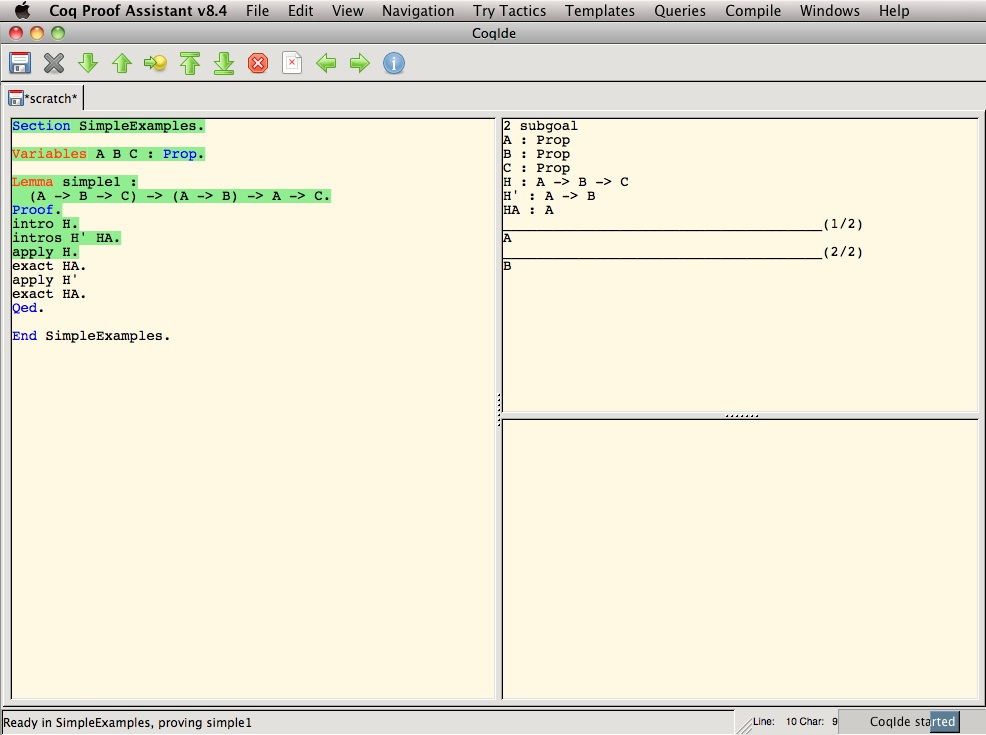
\includegraphics[width=\linewidth]{simple1_1.jpg}
  \caption{CoqIde, displaying the result of entering the tactic ``\texttt{apply H}'' in the top-right panel within the proof of \texttt{(A -> B -> C) -> (A -> B) -> A -> C}.}
  \label{fig:simple1_1}
\end{figure}

\begin{figure}[H]
  \center
  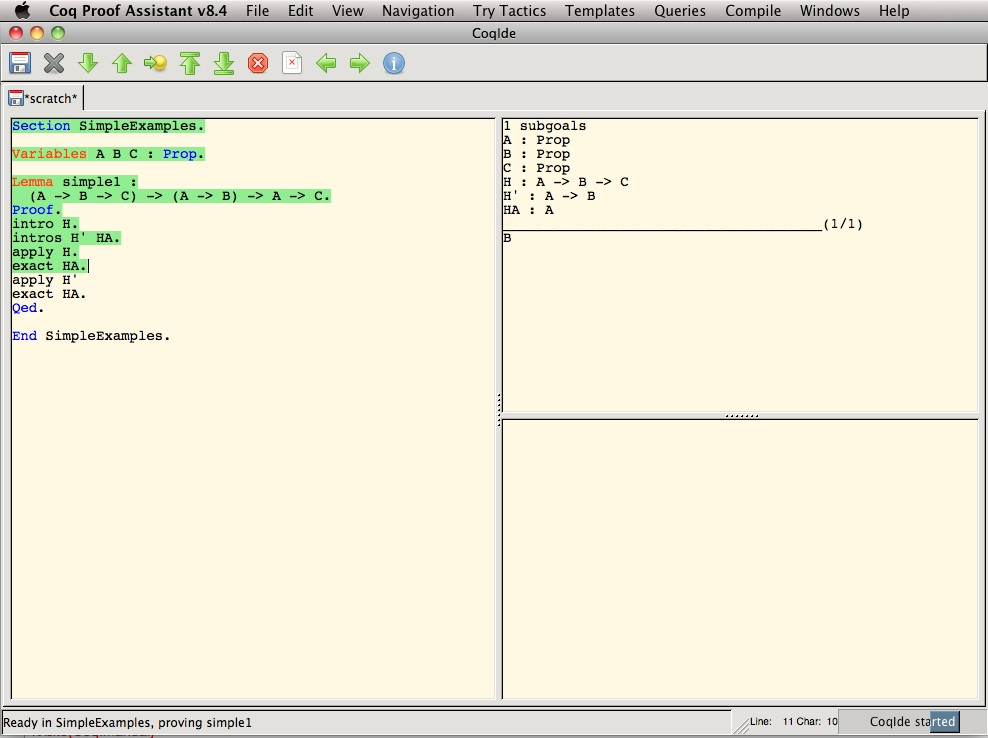
\includegraphics[width=\linewidth]{simple1_2.jpg}
  \caption{CoqIde after moving the end of the evaluated portion of the script forward by one sentence from the state shown in \autoref{fig:simple1_1}.}
  \label{fig:simple1_2}
\end{figure}


Users can extend the highlighted region both forward, to evaluate unhighlighted sentences, and backwards, to undo the effects of evaluation.  Users can instruct the system to extend the highlighting forward by one sentence, to retract it back by one sentence (though in the latest version of Coq, this sometimes will actually move the highlighting back several sentences), to extend or retract it to the cursor, to remove all of it (i.e. retract it to the start of the script), and to extend it to the end of the script.  These instructions can be entered into the system using toolbar buttons, drop-down menu items, or keyboard shortcuts.

\autoref{fig:simple1_1} and \autoref{fig:simple1_2} illustrate some of these points.  In \autoref{fig:simple1_1}, in the top right, we see the the result of evaluating ``\texttt{apply H}''.  In \autoref{fig:simple1_2}, we see the highlighting extended and the result of ``\texttt{exact HA} in the top right, namely the elimination of the first of the two subgoals in \autoref{fig:simple1_1} and the change in focus to the second.

This interface is problematic for novices trying to learn the effects of tactics.  Unfortunately, because the particular example being discussed is so simple, the severity of the problem may not be immediately apparent.  In \autoref{fig:simple1_1}, the two goals resulting from using the tactic ``apply H'' (the statement at the end of the highlighted region) appear to be displayed in the top right panel.  In fact, as mentioned earlier, only the first goal is fully displayed--the context for the second is not.  (In this case, the contexts for both are identical, but this is not always what happens).  To see the context of the second goal, probably the easiest, or at least most natural, thing for the user to do is highlight forward through all the tactics used to prove the first goal (just one tactic here, but potentially many in general).  It is up to the user to determine how far to highlight (or un-highlight, if looking at an earlier sibling goal) by keeping track of the list of goals in the top-right panel.  

In addition to the fact that users must move through the script to fully see siblings, no distinction is made between sibling and non-sibling goals in the list presented.  For instance, instead of using ``\texttt{exact HA}'' to transition to \autoref{fig:simple1_2}, the user could have used a tactic that produced two new goals.  The list of goals would then contain three goals, but only the first two would be siblings.  The user interface leaves it up to the user, however, to determine this by keeping track of the number of goals.\footnote{This sort of debugging gets even harder when one introduces proof automation features that allow combinations of basic tactic use attempts.}

Proof general does introduce a few features not present in CoqIde.  For instance, instead of making the highlighted region un-editable (``locking'' it), typing in the highlighted region retracts the highlighting back to the end of the sentence that is immediately before the cursor.  Unfortunately, these features are not really aimed at showing the effects of tactics.  A third user interface, \textit{Proof Web}\cite{ProofWeb} does make a serious attempt.  ProofWeb, for the most part, is a web-based version of CoqIde.  However, it has a major improvement, shown in the bottom right of \autoref{fig:proofweb}: a visualization of the partially completed proof tree.  

ProofWeb's display of the tree follows the convention where inferences are drawn with a horizontal line separating horizontally listed premises, above, from the conclusion below, and where each horizontal line is labeled with the name of the corresponding inference rule (or, in the case of Coq, by the corresponding tactic name) to the right of the line.  These inferences can be chained together so that the root of the proof tree is drawn at the bottom and the leaves are drawn at the top.  As an example, the portion of the proof tree constructed by ProofWeb that corresponds to ``\texttt{apply H}'' is shown in \autoref{fig:applyH} (the ellipses indicate that the child nodes are still unproved), and \autoref{fig:fulldisplaypartialtree} fully displays the partially completed tree.  The user is able to much more directly see the goal to which \texttt{apply H} is applied and the goals this application produces.

\begin{figure}[H]
  \center
  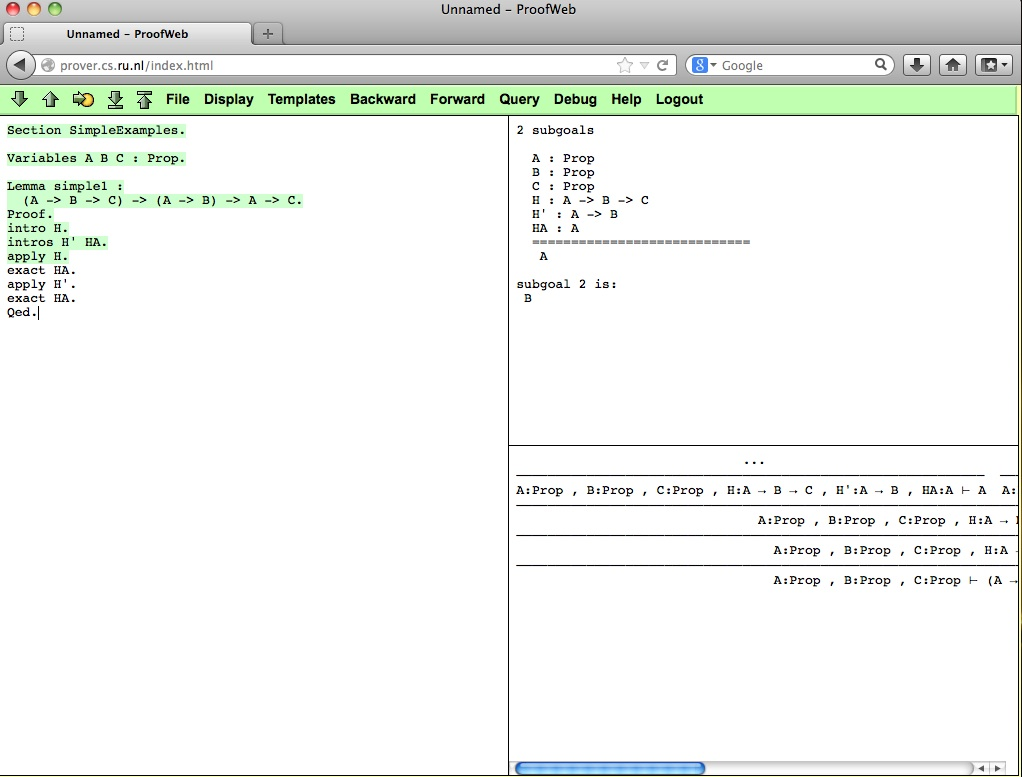
\includegraphics[width=\linewidth]{ProofWeb.jpg}
  \caption{ProofWeb, with a partial proof tree displayed in the bottom right.}
  \label{fig:proofweb}
\end{figure}



Unfortunately, as one can probably already tell, this sort of visualization does not scale particularly well.\footnote{Later in this document I provide what I hope is a clearly better alternative.} Contexts may may have dozens of items, many of which may be much longer than ``\texttt{H : A -> B -> C}, and the number of nodes in the proof tree may also be very large.  As a result, the user may have to pan around the window to see the effect of a tactic; this is especially likely if one is looking at a tactic used near the root of the tree, since the width of the tree at its leaves forces apart nodes near the root.  Even if the user does not need to pan (ProofWeb has a feature that allows the tree to be displayed in a separate window, which can sometimes make panning unneccessary), the distances at which nodes with sibling and parent-child relationships must sometimes be placed may make it difficult for the user to compare such sequents and to determine if a direct relationship in fact exists (e.g. determine if two sequents that are printed next to one another are siblings or ``cousins'').  The latter task is possibly especially difficult using this visualization since it involves checking for gaps in co-linear line segments and the human brain tends to connect such lines.\footnote{This is the Gestalt law of ``good continuation; see, for instance, \cite{field1993contour}.}  The proof tree visualization, especially if there is a need to pan, is also not particularly helpful in showing the location of the current goal (users may have to search the leaves of the tree to find the leftmost ellipsis).

\begin{figure}[H]
  \center
  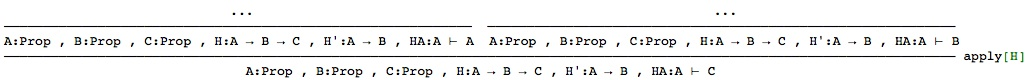
\includegraphics[width=\linewidth]{applyH.jpg}
  \caption{The portion of ProofWeb's tree visualization corresponding to the tactic ``\texttt{apply H}''.}
  \label{fig:applyH}
\end{figure}

\begin{figure}[H]
  \center
  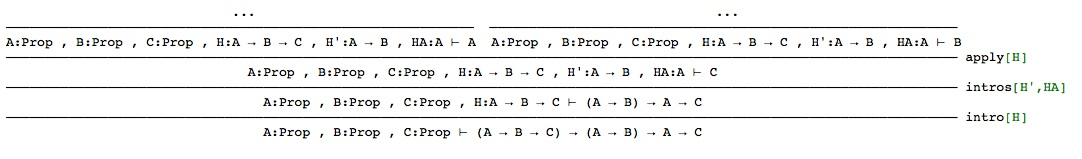
\includegraphics[width=\linewidth]{fullDisplayPartialTree.jpg}
  \caption{The partially completed tree from \autoref{fig:proofweb}, fully displayed.}
  \label{fig:fulldisplaypartialtree}
\end{figure}

The problems with current user interfaces that are discussed above are with respect to the scenario in which a novice user is inspecting an existing proof in order to determine the effects of various tactics under various conditions.  Many other scenarios with overlapping and related challenges also exist.  Such challenges include, but are not limited to,
\begin{itemize}
	\item locating particular items in a context (or in the larger environment)
	\item finding similar nodes in a proof tree
	\item deciding which tactic to apply
	\item keeping track of different proof attempts
	\item optimizing a proof or organizing a set of definitions, theorems and proofs for human understanding
	\item doing all these things efficiently. 
\end{itemize}



%%================================
\section{Coq User Interface Survey}
%%================================
Section \ref{currentUIproblems} described some usability problems that I, as a novice Coq user, noticed.  In this section, I describe an online survey (and its results) that Professor Juan Pablo Hourcade, Professor Aaron Stump, and I, in December 2011, invited subscribers to the Coq-Club mailing list to fill out.  This survey asked Coq users for their opinions and experiences regarding existing Coq user interfaces, and for their ideas regarding new interfaces.  Our motivation was both to validate our own ideas about new Coq user interfaces and to generate new ones.  We received 48 responses, including many detailed responses to the essay questions in the survey.

The survey consisted of 19 questions, of which 13 were multiple choice and the rest short answer or essay. The questions can be divided into three groups:  7 questions asking for background information on the respondent and how the respondent uses Coq, 9 questions asking for various ratings of the interface respondents use, and 3 open-ended questions directly related to the development of new user interfaces.  To these open-ended questions, we received many lengthy and thoughtful responses. \footnote{A more detailed survey report can be found at http://www.cs.uiowa.edu/~baberman/coquisuvey.html.}

The responses to the first group of questions showed a full range of (self-reported) Coq expertise levels, although a majority of responses indicated a high degree of expertise (on a scale going from 1=�novice� to 5=�expert�, 2 respondents rated themselves at level 1, 12 at level 2, 9 at level 3, 17 at level 4, and 8 at level 5).  9 respondents indicated they had been using Coq for less than 1 year, 27 for 1-5 years, 7 for 5-10 years, and 5 for more than 10 years.  Users of Proof General outnumbered users of CoqIDE 31 to 16.  24 respondents indicated using Coq for programming language or program verification research, 10 indicated using Coq for formalization of mathematics, and 8 indicated �teaching.� 

In the second group, to the question ``How satisfied are you with the interface you typically use?'', respondents gave a slightly positive average response (4.6 on a 1 to 7 point scale).  This was somewhat surprising to us at first, but it may have been an artifact of how the the question was asked.  For one thing, we did not present any sort of alternative interface, and current interfaces are, in fact, a significant improvement over the basic command prompt.  A second factor may be that many respondents have become accustomed to their current interface and may have viewed the question as asking how willing they would be to learn to use a new interface.  More than 25\% of respondents, however, did indicate some level of dissatisfaction.  Furthermore, answers to four questions revealed difficult tasks for users.  These questions asked users how difficult it is, using the interface they typically use, to 
\begin{itemize}
\item understand the relationships between subgoals, 
\item switch back and forth between potential proofs of a subgoal, 
\item compare similar subgoals, and 
\item tell what options for proving a subgoal are available. 
\end{itemize}
On a scale where 1=``Very Difficult'' and 7=``Very Easy'', the mean values for the answers to these questions were 2.74, 3.46, 2.35, and 2.57, respectively.   Responses to a fifth question, �How difficult is it for you to (mentally) parse Coq syntax?�, produced a mean value of 5.02 on the same scale, with only 4 responses indicating �Difficult� or �Somewhat difficult�.  Again, this may have been an artifact of the way the question was asked--how difficult, compared to what?

In the third group, we received almost 4,500 words (total) in response to the questions  
\begin{itemize}
\item ``What information would you like to have more readily available when working with Coq?'',
\item ``What do you think are the hardest parts of learning interactive theorem proving with Coq?'', and
\item ``What advice/requests/ideas do you have for creating better Coq user interfaces?''
\end{itemize}
Because of this volume, I (very roughly) categorized the responses to each question.

For the first question, the first category was ``library documentation.'' Respondents noted that Coq's ``\texttt{SearchAbout}'' command is a little hard to use, that they would like more simple examples of using Coq commands, that theorem names are not very readable, and that they would like integration of documentation, a la the Eclipse IDE's javadoc support.\footnote{For the reader not familiar with Integrated Development Environments, they are essentially text editors with features specialized to programming in various languages.  Eclipse\cite{Eclipse} is one of the more popular IDEs for Java programming.}  The second category was ``available tactics''/``relevant lemmas, relevant definitions'': respondents wanted the names of previously proved statements they could apply and, additionally, whether a tactic could be used to automatically prove either the the current goal or its negation.  The third category was information on terms, e.g. the type of a term, the value to which it reduces, or other implicit information (such information can already be made available by using commands like ``\texttt{Check}'' and ``\texttt{Print}'').  The fourth category was proof structure, including information on the relationships both between goals within a proof and between theorems and definitions.  Miscellaneous responses included similarities between terms, differences between terms and expected terms, and tactic debugging with custom breakpoints.

For the question ``What do you think are the hardest parts of learning interactive theorem proving with Coq?'', the first category of response was type theory-- that learning the type theory behind Coq is one of the hardest parts.  The second category was with lack of good tutorials.  The third category was that there are numerous poorly documented commands (the need for simple examples was mentioned again).  Finally, the fourth category was proof readability, e.g. lack of support for mathematical notation and proof script organization.

For the question ``What advice/requests/ideas do you have for creating better Coq user interfaces?'', the first category was programming IDE features (e.g. auto-indentation, safe and correct renaming of identifiers, refactoring of tactics and groups of tactics, and background automation).  The second category was proof structure: representing proof structure by for instance grouping sibling goals, and allowing more flexibility to the order in which one works on goals.  The third category was syntax, which included having better ways to indicate where one wants to rewrite part of a term or where one wants to unfold a definition and automatic naming of hypotheses.  Some miscellaneous suggestions were to make more use of the mouse, avoid unnecessary re-execution of potentially long-running commands, and to have different editing and presentation tools.   

Even given the responses from self-described novice Coq users, the group of respondents is still heavily biased towards acceptance of arcane, complicated software.  The responses summarized above demonstrate that, even by this group, room for improvement is seen.

%%=======================================================================================
\chapter{Proposed and Completed Research}
%%=======================================================================================
%%================================
\section{Overview}
%%================================

In this section, I describe CoqEdit, three extensions to CoqEdit, and plans for evaluating two of these extensions with human participants.  As an interlude in the descriptions of the extensions, I include a presentation of the development and testing of ``Keyboard-Card Menus'' as these are a component of one of the planned extensions.

%%================================
\section{CoqEdit}
%%================================

CoqEdit is a new user interface of Coq, that I, along with Harley Eades and under the supervision of Professors Juan Pablo Hourcade and Aaron Stump, have been developing. CoqEdit is a plugin to the \textit{jEdit}\cite{jEdit} text editor, a free and open source editor editor written in Java.\footnote{Another jEdit plugin, \textit{Isabelle/jEdit}, has been developed to provide support for the Isabelle\cite{Isabelle} interactive theorem prover and is bundled with Isabelle itself; see, for instance, \cite{wenzel2012asynchronous}.  Note that it has a rather different, and arguably more advanced, ``asynchronous'' style of interaction.  While this style of interaction may one day be available to Coq users, for now we are concentrating on other issues.}  For the most part, interaction with CoqEdit, at least in its unextended form, imitates the style seen with Proof General and CoqIde.  

\autoref{fig:coqedit} shows an initial version of the plugin.  This initial version is functional in that one can communicate with the \texttt{coqtop} command prompt by moving the highlighting forwards and backwards (using submenu items not seen in figure 6, or the items' shortcuts) to send messages to \texttt{coqtop}, which can then respond by changing the text printed in the two panels on the right.  It also allows allows \texttt{coqtop} to be interrupted when processing long-running commands, and includes the XML files telling jEdit how to do syntax highlighting for Coq's .v (``Vernacular'') files.  Note that these two panels actually sit within a jEdit ``dockable window'', which may be hidden (i.e. collapsed so that only its labeling tab is showing), undocked (i.e. made to float as a normal window), or docked in some other position (e.g. below the area containing text, instead of to its right).

\begin{figure}[H]
  \center
  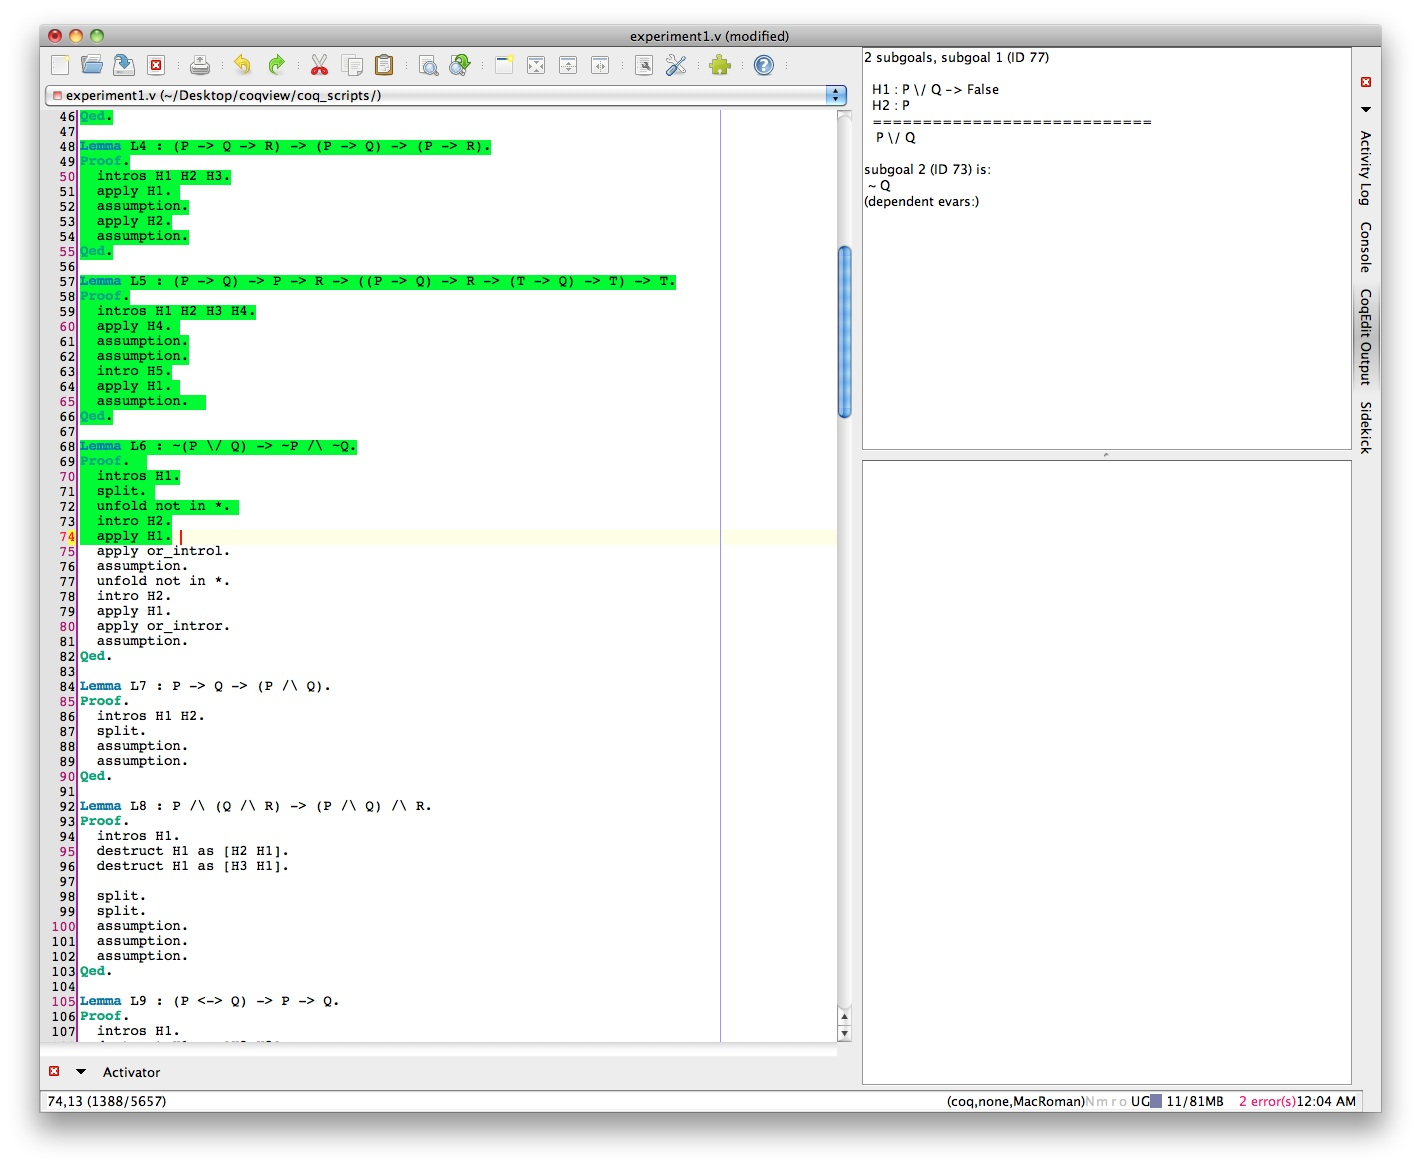
\includegraphics[width=1.1\linewidth]{coqedit.jpg}
  \caption{An initial version of CoqEdit.}
  \label{fig:coqedit}
\end{figure}

Although it does not contain some of the language-specific features of IDEs like Eclipse, jEdit does contain several noteworthy ones, besides its support for plugins.  These include syntax highlighting and auto-indentation for numerous languages, word completion, abbreviations, folding and many others (see the jEdit homepage\cite{jEdit}, and the features page to which it links).  The fact that jEdit runs on a Java Virtual Machine allows it to be used with Mac OS X, OS/2, Unix, VMS and Windows, and should also make extending CoqEdit support to multiple platforms relatively easy (I am currently developing it just under Mac OS X, but I expect it to immediately work just as well on Linux). Particularly important for the development of plugins is its BeanShell scripting language for writing macros, essentially an interpreted version of Java that makes experimentation with the jEdit API relatively easy, especially for Java programmers.  Plugins are, for the most part, actually collections of BeanShell scripts that generally invoke compiled Java code.

One of the features of jEdit's plugin system is that one can specify dependencies between plugins.  If plugin \textit{A} is specified as depending on plugin \textit{B}, then activating\footnote{``Loading'' a plugin does not necessarily ``activate'' it.}  \textit{A} in the plugin manager automatically activates \textit{B}.  This allows code from \textit{B} to be invoked from \textit{A}.  This makes it possible to write extensions to CoqEdit as jEdit plugins that allow features to be added incrementally and in various combinations.  In a nutshell: we can write plugins that plug into our CoqEdit plugin.

Currently, I am working on a major revision of the initial version shown in \autoref{fig:coqedit}.  Although this revision will include bug fixes and implement a few remaining unimplemented features, its main purpose is to improve the software architecture in order to make future CoqEdit extensions easier.  \textit{This foundation for future user interface research will be one of the major contributions involved in this dissertation.}  It will make taking advantage of the extensive Java libraries, particularly those for 2D graphics, and of the Java development community's expertise, much more straightforward.

This new, still quite basic, user interface will however improve upon Proof General and CoqIde in a couple of different ways.  First, it will cache the output of sentence evaluation and allow a window into this cache using movable dark green highlighting of a sentence within the evaluated region (Proof General caches this output, but requires users to hover over the text with the mouse to make a tooltip with the output appear).  Second, it will allow both multiple instances of \texttt{coqtop} to run simultaneously \textit{and} multiple text areas to show multiple areas within a buffer that is being evaluated (CoqIde allows only the former and Proof General allows only the latter). 


%%================================
\section{CoqEdit Extensions}
%%================================

%%============
\subsection{``Proof Previews''}
%%============

Our first experimental extension, ``{\bf Proof Previews}'', is shown in \autoref{fig:proofpreviews}.  When the user presses CTRL-SPACEBAR while the system is in proof mode, a popup window containing a list of possible tactic/argument combinations (i.e. ones that do not immediately produce errors or take especially long to run) appears just below the end of the evaluated section.  The user can use the up and down arrow keys to change the selected item in the list and the ENTER key to insert the selected item into the script.  In addition, the output that would result from evaluating the selected item is displayed in the bottom output panel.  The general goal of this plugin is to allow users, novice users in particular, to quickly explore their available options.


\begin{figure}[H]
  \centering
  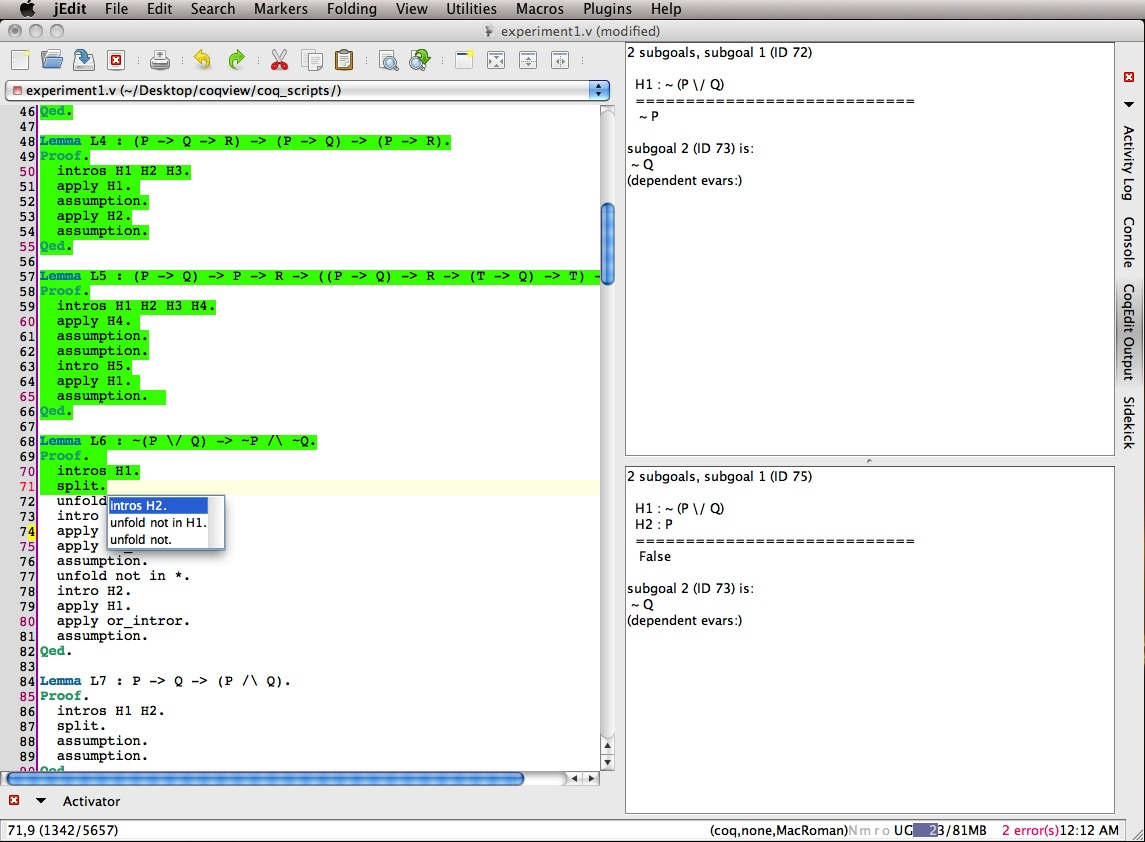
\includegraphics[width=1.1\linewidth]{proofpreviews.jpg}
  \caption{The initial version of CoqEdit with the Proof Previews extension.  The result of the highlighted tactic is displayed in the bottom output panel.}
  \label{fig:proofpreviews}
\end{figure}

The tactic list generation capabilities for this plugin are quite limited at the moment:  only tactics used in propositional logic exercises and examples may appear in the list.  While this may still be useful for educational purposes, our implementation is mainly to be used for usability testing and to demonstrate the utility of the general idea.  A more fully developed version of this plugin would be possible, but would likely require some quite complicated indexing of Coq's standard library.  

%%============
\subsection{``Proof Transitions''}
\label{prooftransitions}
%%============

Our second experimental extension, ``{\bf Proof Transitions}'', evolved from two separate ideas.  The first is {\bf proof tree visualization}.  Originally, we proposed visualizing Coq's proof trees as in \autoref{fig:prooftreebuild}, where 
\begin{itemize}
\item the red half circles represent goals, 
\item the blue half circles, placed on top of the red half circles to form complete circles, represent tactics successfully used with the goals corresponding to these red half circles, 
\item child goals are arranged \textit{above} parent nodes (as in \autoref{fig:fulldisplaypartialtree}),
\item thin red lines connect parent nodes to unproved child branches, 
\item thick black lines connect parent nodes to proved child nodes, and
\item the yellow arrow represents the current node.
\end{itemize}
(\autoref{fig:prooftreebuild} visualizes the example from section \ref{examplesection}).

In addition to helping users in seeing which child goals are associated with which parent goals and tactics, and potentially in traversing/adding to the trees' nodes in arbitrary orderings, this sort of visualization could be enhanced further to provide valuable information.  For instance, \autoref{fig:similarnodes} shows nodes being highlighted based on similarities in the tactics \footnote{...which might be particularly helpful in avoiding loops proofs}.  The information associated with these nodes could be compared side-by-side using an additional output window whose location within the proof tree could be represented by an additional arrow, as in \autoref{fig:nodecomparison}.  

\begin{figure}[H]
  \center
  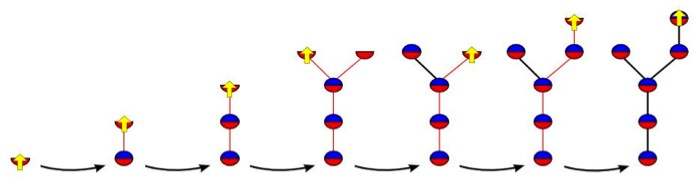
\includegraphics[width=1.1\linewidth]{prooftreebuild.jpg}
  \caption{A series of partial proof tree visualizations of the example of section \ref{examplesection}, in an earlier style.  }
  \label{fig:prooftreebuild}
\end{figure}

\begin{figure}[H]
  \center
  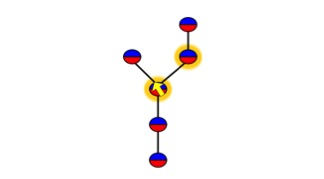
\includegraphics[width=0.7\linewidth]{similarnodes.jpg}
  \caption{Similar nodes being highlighted while the node under the yellow arrow is inspected.}
  \label{fig:similarnodes}
\end{figure}

\begin{figure}[H]
  \center
  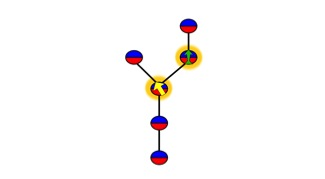
\includegraphics[width=0.7\linewidth]{nodecomparison.jpg}
  \caption{The proof tree visualization of \autoref{fig:similarnodes}, with an additional arrow to represent the location of another output window within the proof tree.}
  \label{fig:nodecomparison}
\end{figure}

Proof tree visualizations could also be enhanced to support management of different versions of proof tree branches, as in \autoref{fig:versionmanagement}, and to support proof presentation, as in \autoref{fig:presentationmanagement} which shows how a branch deemed uninteresting might be removed from the visualization.  These examples suggest the existence of a wide range of possible user interface improvements that may not even have been thought of yet, and that are part of the rationale for making CoqEdit more easily extendable.

\begin{figure}[H]
  \center
  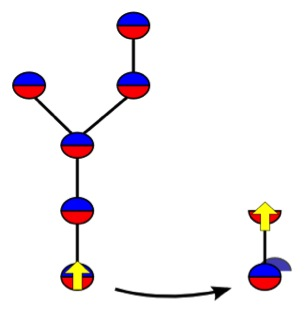
\includegraphics[width=0.35\linewidth]{versionmanagement.jpg}
  \caption{A user might decide to try an alternate proof of a branch of the tree (the branch could be, as in this case, of the entire tree).  A saved copy of the original branch might be represented by a ``shadowing'' blue half-circle, as seen on the right-hand side of this figure.}
  \label{fig:versionmanagement}
\end{figure}

\begin{figure}[H]
  \center
  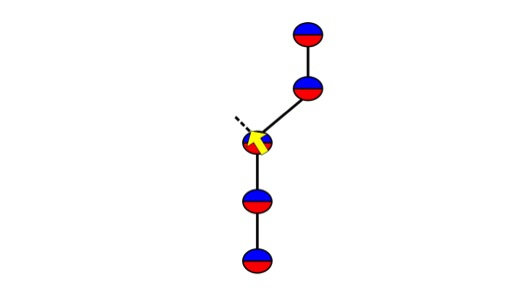
\includegraphics[width=0.7\linewidth]{presentationmanagement.jpg}
  \caption{The visualization of \autoref{fig:similarnodes}, with a branch hidden.  This sort of hiding might be useful in making the structure of the remaining visible branches more clear.}
  \label{fig:presentationmanagement}
\end{figure}


The second idea from which the Proof Transitions extension evolved was ``{\bf Inference Rule Highlighting}''.   The idea here is to use highlighting the to show the pattern, or inference rule, being instantiated by a tactic application to a goal.  In \autoref{fig:inferenceruleinstance}, we see an instance of the general rule seen in \autoref{fig:inferencerule}.  The blue box contains a tactic while the red box below contains the old goal and the red box above contains the new goal (with other tactic applications, one might see several red boxes above).  The more general goal is to help expert users debug proof scripts and to help novice users gain an intuition for how specific tactics work.


\begin{figure}[H]
  \center
  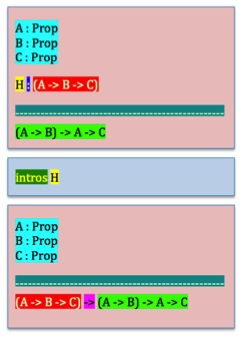
\includegraphics[width=.40\linewidth]{inferenceruleinstance.jpg}
  \caption{Inference Rule Highlighting example:  child, parent, and tactic, with highlighting showing where the tactic has moved and added text.}
  \label{fig:inferenceruleinstance}
\end{figure}
s

\begin{figure}[H]
  \center
  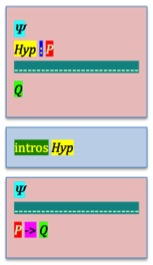
\includegraphics[width=.25\linewidth]{inferencerule.jpg}
  \caption{The general inference rule on which \autoref{fig:inferenceruleinstance} is based.}
  \label{fig:inferencerule}
\end{figure}


This particular way viewing the effects of tactics may work for many of the basic tactics, but it does not scale very well to more complicated tactics, since, for one thing, one eventually runs out of easily-distinguishable colors and, moreover, many tactics do not correspond to patterns like that seen in \autoref{fig:inferencerule} (e.g. the \texttt{auto} tactic that tries to automatically prove a goal).  Proof Transitions will provide an alternative which, in an initial form, can be seen demonstrated in \autoref{fig:pt1}, \autoref{fig:pt2}, \autoref{fig:pt3}, and \autoref{fig:pt4}.  \autoref{fig:pt1} shows the initial goal.  \autoref{fig:pt2} shows how immediately after the tactic \texttt{intros H1 H2} has been processed by the system, a blue box, containing the tactic, is placed immediately on top of the old goal and the new goal, in another red box, is placed further up with a line connecting its red box and the blue box.  As an option, as seen in \autoref{fig:pt3}, highlighting and underlining can be added to the boxes' text according to the following rules:  
\begin{itemize}
\item red highlighting in the bottom red box to show text that is deleted altogether, 
\item green highlighting in the top red box to show text that is entirely new, 
\item yellow highlighting in any box to show text that is moved (or copied, in the case of identifiers given as the tactic arguments),
\item red underlining in the bottom red box to show text that is either moved or deleted altogether, and 
\item green underlining in the top red box to show text that is new (either entirely new or moved/copied into the box)
\end{itemize}
In addition, the user can have lines drawn to connect the moved/copied portions of text, as seen in \autoref{fig:pt4}.  Note that the lines are actually drawn one-by-one in an animation, which makes it easier to see what is connected to what than might appear to be the case just looking at \autoref{fig:pt4}.  As an alternative to drawing lines, the yellow-highlighted text might be made to float up to the new positions.  Note also that this extends the sorts of visualizations one commonly sees of the \textit{UNIX} \texttt{diff} command\footnote{\texttt{diff} is used to find changes between versions of text files}:  instead of just indicating what text has been added, what removed, and what changed, we also show what has been moved or copied.  Consequently, it would seem likely that variations of the idea might be applied in numerous other coding environments.

\begin{figure}[H]
  \center
  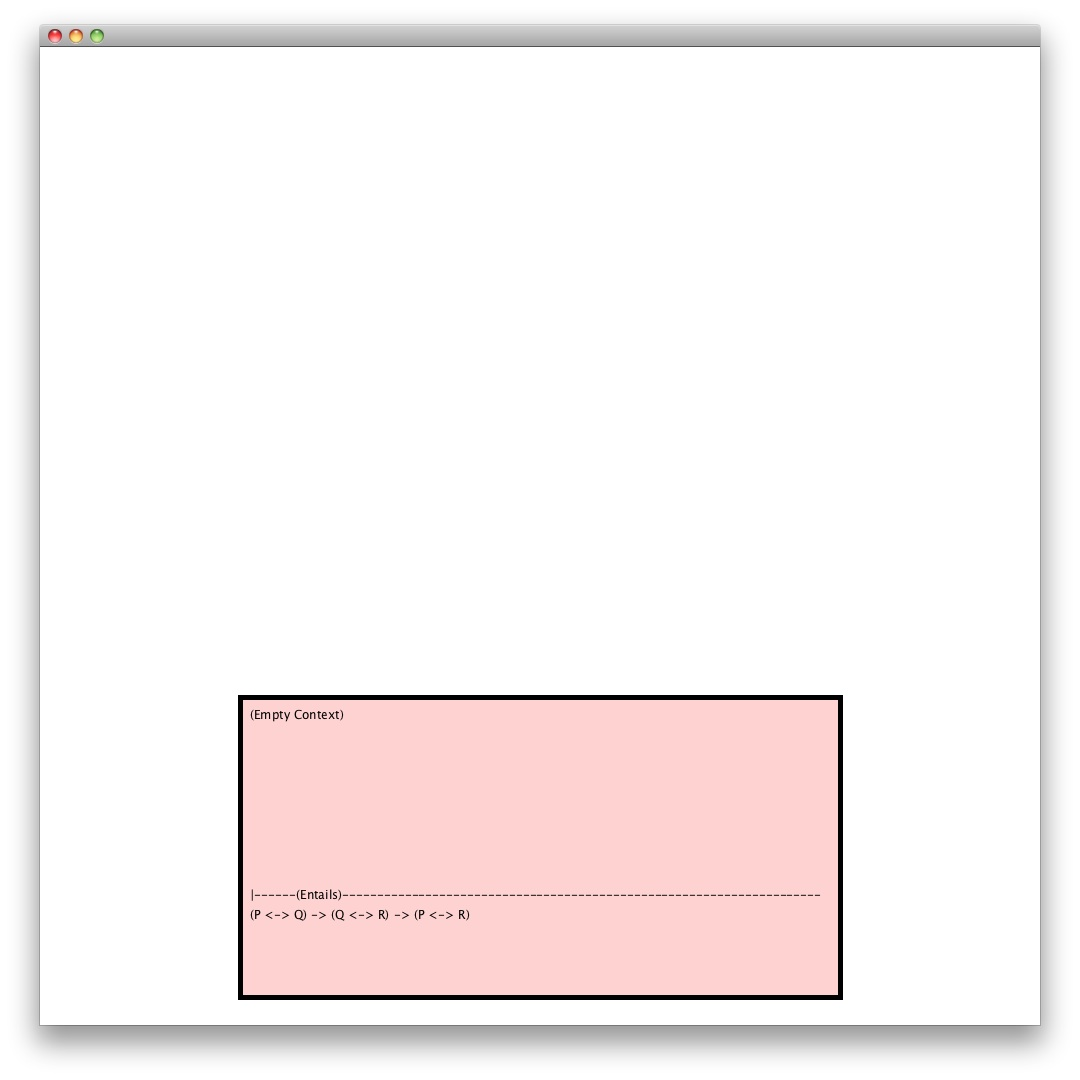
\includegraphics[width=\linewidth]{pt1.jpg}
  \caption{Proof transitions: a goal, pre-transition}
  \label{fig:pt1}
\end{figure}

\begin{figure}[H]
  \center
  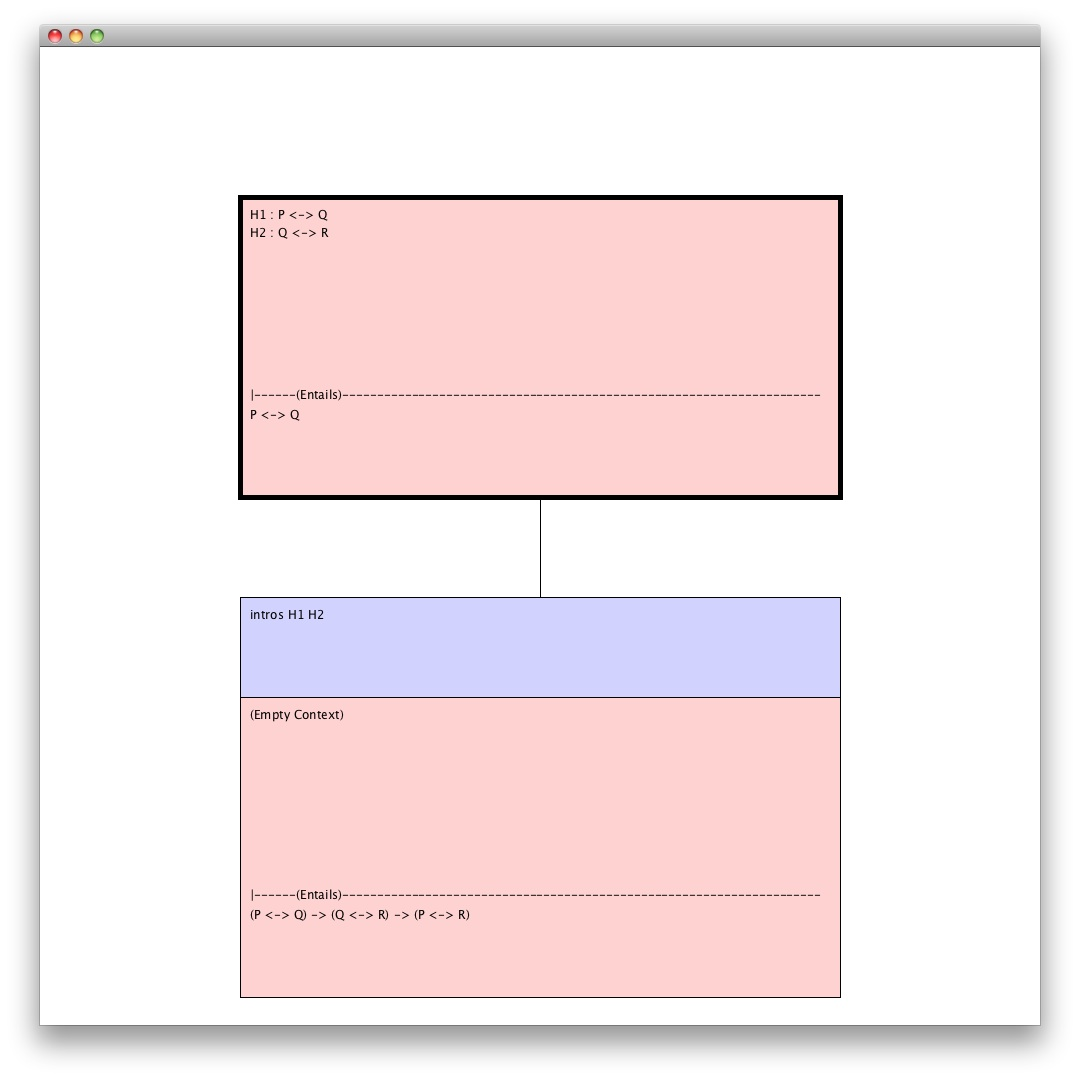
\includegraphics[width=\linewidth]{pt2.jpg}
  \caption{After a tactic has been applied to the goal in \autoref{fig:pt1}.}
  \label{fig:pt2}
\end{figure}

\begin{figure}[H]
  \center
  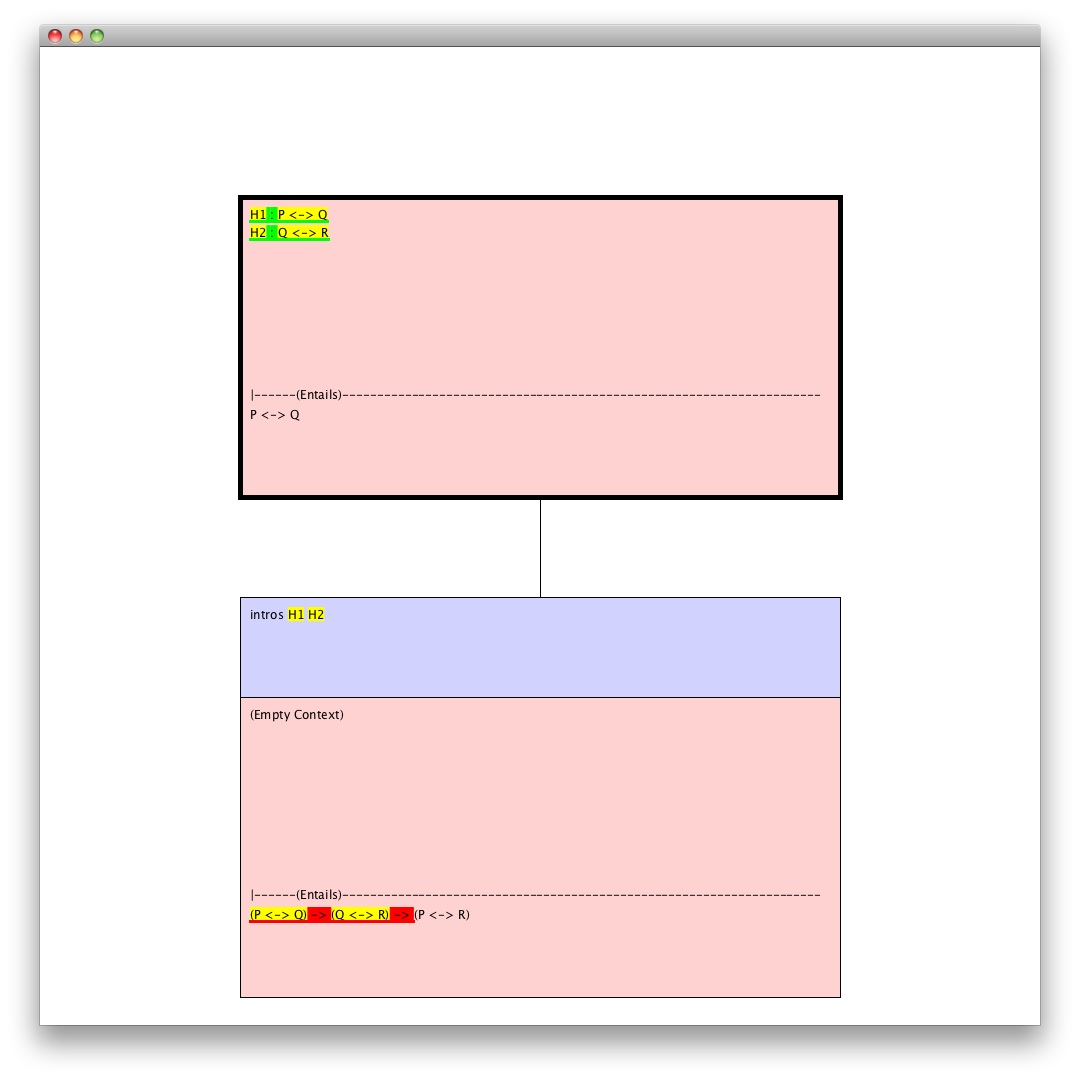
\includegraphics[width=\linewidth]{pt3.jpg}
  \caption{\autoref{fig:pt2}, with highlighting to show changed text.}
  \label{fig:pt3}
\end{figure}

\begin{figure}[H]
  \center
  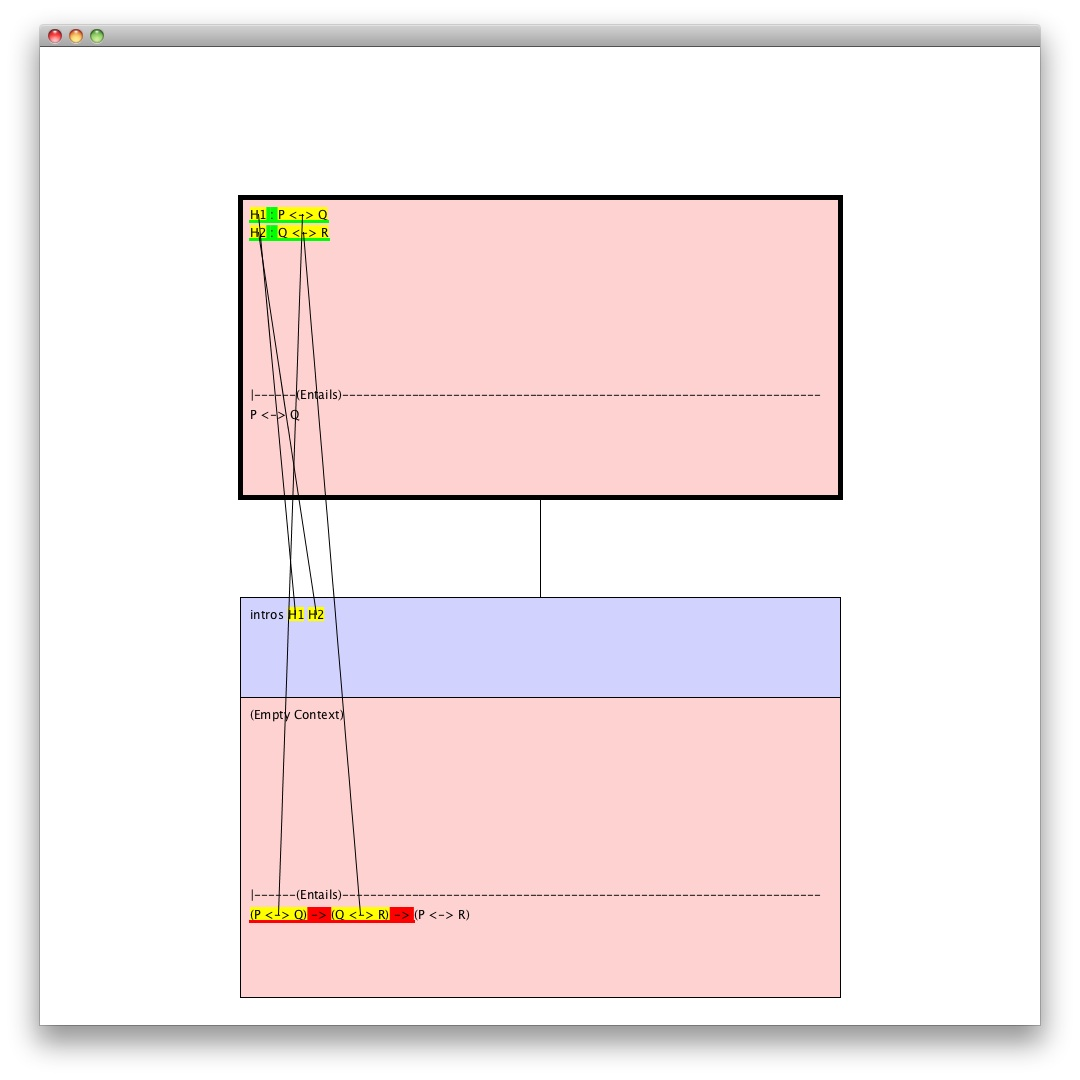
\includegraphics[width=\linewidth]{pt4.jpg}
  \caption{After a tactic has been applied to the goal in \autoref{fig:pt1}, stage 3.  Note that the lines would be added one at a time.}
  \label{fig:pt4}
\end{figure}

Because development of this plugin is being done using the \textit{Piccolo}\cite{Piccolo2D} toolkit for ``structured 2D graphics'', which provides support for ``zoomable user interfaces'', it will be relatively easy to also provide support for proof tree visualization.  \autoref{fig:ptZoomOut} shows what zooming out from \autoref{fig:pt2} might look like if the two boxes were the root and its first child and another two lines were leaving the tactic.  \autoref{fig:ptZoomOut2} shows the proof tree of \autoref{fig:ptZoomOut} with the second child node of the root node set as the current node; note how one can automatically adjust the layout of the tree based on the requirement that the current node be centered above its parent (if the current node is not the root, of course) and without a lot of change in the layout of the branches.   

\begin{figure}[H]
  \center
  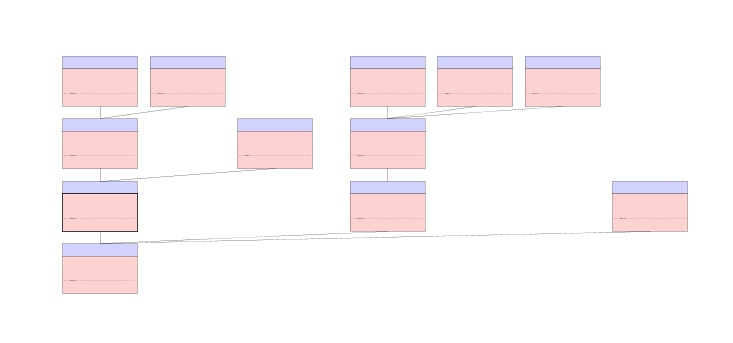
\includegraphics[width=\linewidth]{ptZoomOut.jpg}
  \caption{The boxes of \autoref{fig:pt1}, \autoref{fig:pt2}, \autoref{fig:pt3}, and \autoref{fig:pt4},  as part of a proof tree visualization.}
  \label{fig:ptZoomOut}
\end{figure}

\begin{figure}[H]
  \center
  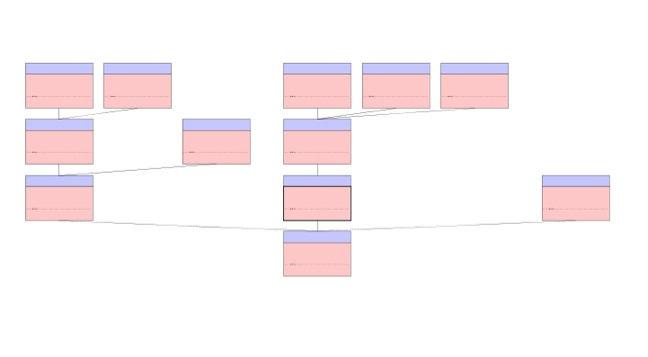
\includegraphics[width=\linewidth]{ptZoomOut2.jpg}
  \caption{The tree of \autoref{fig:ptZoomOut}, laid out with the root node's second child, instead of its first, set as the current node}
  \label{fig:ptZoomOut2}
\end{figure}

Please note that this design of this extension is likely to change significantly in the future, and that for the purposes of this dissertation I am likely only to produce a ``Wizard of Oz'' version for user testing purposes.  More specifically, I will be producing a pair of plugins that simulate an actual Proof Transitions extension acting on a particular pair of proof scripts. For a real version of the plugin, it would probably make sense to have more support in the \texttt{coqtop} back end for these features beforehand, particularly with regards to determining which portions of goals are moved.  One purpose for developing these plugins is to demonstrate that such support ultimately would be useful.

%%================================
\subsection{Interlude: Keyboard-Card Menus}
%%================================

In this section, I describe work on ``Keyboard-Card Menus'', which I hope to incorporate into a third extension to CoqEdit.  The contents of this section is to be presented at the Interaccion 2013 conference and published in its proceedings under the title \textit{Keyboard-Card Menus: Faster Learning of Many Fast Commands}.  It was written by myself and my advisor, Professor Juan Pablo Hourcade, at the University of Iowa.

\subsubsection{Abstract}  We present a study comparing ``keyboard-card'' menus' presentation of non-traditional shortcuts with a presentation of these same shortcuts that uses dropdown menus.  Keyboard-card menus are a new type of menu system in which potentially hundreds of menu items are arranged in sets of keyboard patterns that are designed to be navigated using only a computer keyboard's character keys, for fast access.  In selecting items from these menus, novice users physically rehearse the same actions that an expert would use.  The data from our study shows that keyboard-card menus have significant advantages over dropdown menus in making the transition to expert use faster.

\subsubsection{Introduction}

Keyboard-card menus are a new type of menu we have developed which present menu items in a computer-keyboard shaped arrangements.  They are designed to be navigated using the keyboard, and in doing so users end up learning shortcuts. Our testing shows significant advantages over a presentation of these same shortcuts that uses dropdown menus.   Our ultimate goal in working on keyboard-card menus  is to develop a system that avoids making tradeoffs between three properties:  how easy the system is to learn, how efficiently experts are able to select menu items, and how many menu items are easily accessible.  

While widely-used interaction techniques often support two of these three properties, they do so at the expense of the third, which can be considerably limiting for certain tasks and people.  Consider an example we had in mind while developing the menu:  undergraduate college students writing and manipulating mathematics.  Many of these students do not have the time to learn an unfamiliar, non-WYSIWYG (what-you-see-is-what-you-get) system like \textit{LaTeX}, but also need an efficient system since they are asked to write many equations in homework assignments (especially if they are asked to ``show their work"), \textit{and} they need to be able to access many mathematical symbols.  Handwriting recognition systems might be much easier to learn, but even if the system's recognition accuracy is 100\%, in our opinion handwriting speed is a low bar for efficiency (14 to 15 year old students' handwriting, when copying, has been measured as averaging only 118 characters per minute or, at 5 characters per word, 24 words per minute \cite{graham1998development}).  WYSIWYG systems like \textit{Mathematica} and Microsoft \textit{Word}'s equation editor allow use of either the mouse or keyboard shortcuts to select symbols from menus and toolbars.  While this might be seen as supporting both novice and expert users, since keyboard shortcuts can provide speed advantages once learned, it has been shown that, in general, many users never make the transition to using shortcuts, even in heavily used applications like \textit{Word} \cite{Lane05}.

Writing and manipulating mathematics is not the only application where the users would need to be quickly trained to efficiently select from a large number of menu items.  Novice writers of other sorts of code could benefit as well; for instance, novice HTML coders must spend considerable time learning which tags to select from the large number available.  We suspect that there are many other sorts of activities, particularly in data entry, classification, and retrieval, that could be made more practical by supporting a better balance between efficiency and learnability in applications where items must be selected from a large pool. 

In the next section, we describe how keyboard-card menus present menu items, how they are navigated, and some related work.  We go on to describe our study, which compared keyboard-card menus with dropdown menus, and discuss its results, which show significant advantages for keyboard-card menus. 
Keyboard navigation for keyboard-card menus (and keyboard navigation for the dropdown menus in our study) is unusual in that users are required to press and hold character keys (i.e. to use the character keys themselves as modifier keys); we call these interactions ``rolled-chords,'' or ``rolled-chord shortcuts''.  We therefore include a discussion of the advantages and disadvantages of this approach relative to other ways the keyboard might be used in navigating the menus.

\subsubsection{Keyboard-Card Menu Design:  Keyboard-Card Menus}

Inspired in part by work on keyboard-based menus for wearable computers, seen in \cite{Lyons03}, we have developed keyboard-card menus which lay out menu items in keyboard patterns that \textit{show} users what keys to press, instead of simply listing menu items with shortcut key names; in principle, at least, users do not even need to know the name of the key they want to press.  (An example keyboard-card menu--one used in the study described below--is shown in the lower half of \autoref{fig:kcmidahooxford}, and in \autoref{fig:kcmoxfordzoom}).   

More specifically, the menu system consists of colored ``keyboard-cards'', each of which serves as a submenu (except for one card that serves as a root menu).  Each keyboard-card has printed on it a set of squares arranged in a keyboard pattern.  Printed on top of some (potentially all) of these squares are the menu items that can be selected by pressing the corresponding keys.  To make the affordances of the menu system more obvious to users, squares with menu items are also a lighter color than the rest of the card and each square corresponding to a submenu has an arrow in the bottom right corner.  As a secondary mechanism for associating the menu item with the key, and to make it even more obvious to users that they should use the keyboard rather than the mouse, each square with a menu item also has the corresponding key's character printed in white in a large font, behind the menu item text.


\begin{figure} [H]
  \center
  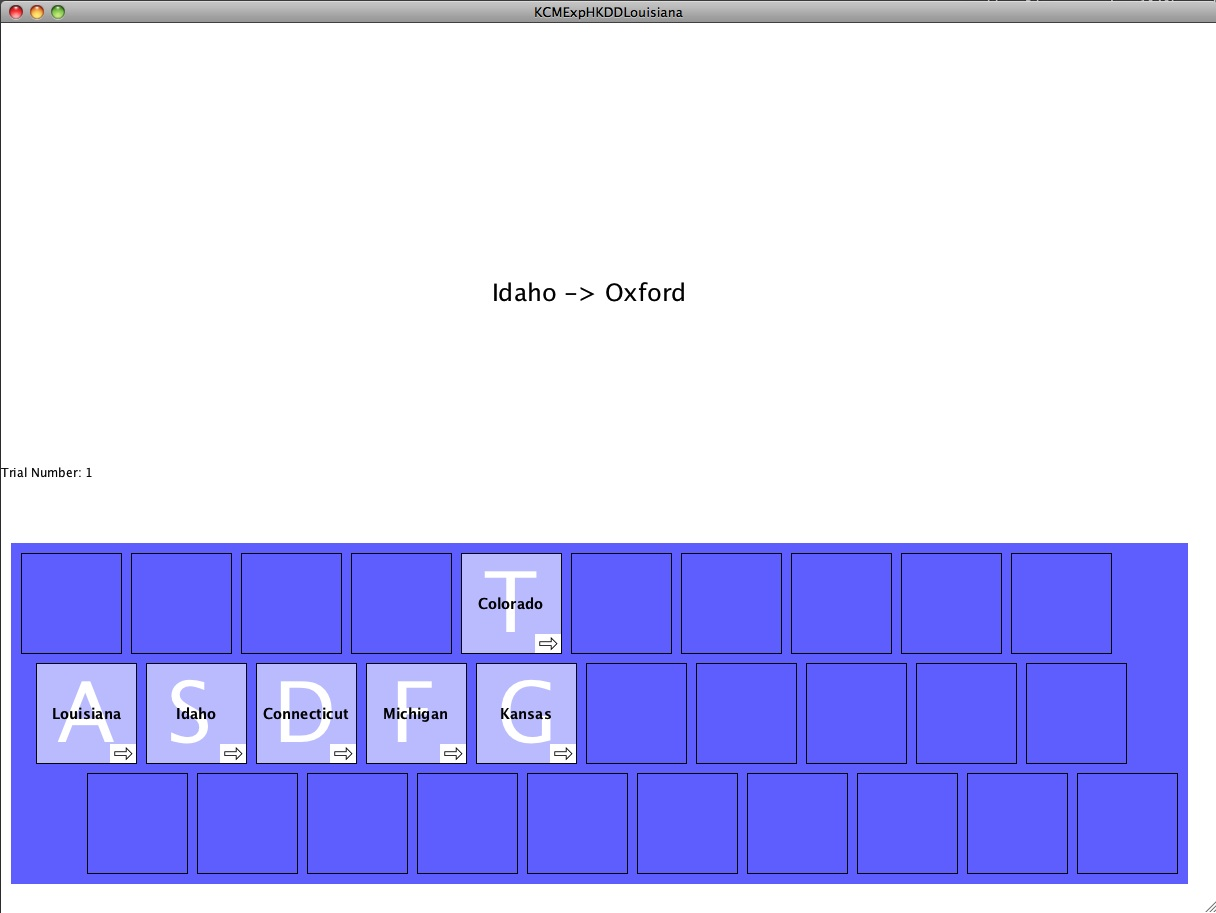
\includegraphics[width=\linewidth]{KCMIdahoOxford.jpg}
  \caption{One of the two keyboard-card menu root cards used in the study, with a prompt for the participant.  A small arrow in the corner of each key indicates that there is a submenu associated with that key.  Participants in the study did not have to rely on this design detail.}
  \label{fig:kcmidahooxford}
\end{figure}

\begin{figure} [H]
  \begin{center}
  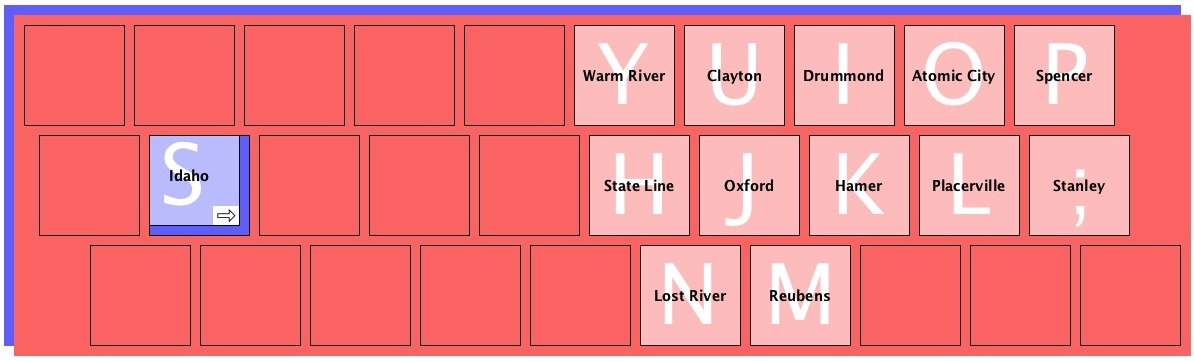
\includegraphics[width=\textwidth]{KCMOxfordZoom.jpg}
  \caption{The keyboard-card menu from \autoref{fig:kcmidahooxford} with the S key pressed.  Note how a hole has been ``punched out'' of the card.}
  \label{fig:kcmoxfordzoom}
  \end{center}
\end{figure}

Initially, when no keys are pressed, only the root card, with top-level menu items, is visible (as in the lower half of \autoref{fig:kcmidahooxford}).  Whenever a key corresponding to a submenu (rather than a leaf in the hierarchy) is pressed--\textit{and held down}--that submenu's keyboard-card is placed on top of the existing card(s), slightly offset to show the number of keyboard-cards below it (as in \autoref{fig:kcmoxfordzoom}, which would be displayed while the S key is held down).  Releasing that key hides that keyboard-card again. (Although the issue was ignored in our study, since no more than two cards, including the root card, were ``stacked'' at a time, releasing a key to hide a keyboard-card would most likely also just hide any cards on top of it, even if the keys associated with those cards were still pressed).  Holding down a key corresponding to a leaf in the menu hierarchy, in addition to performing whatever action is assigned, thickens the outline of the corresponding square on the fully-visible top card.

Because menu item selection is performed entirely from the keyboard, without the user having to move his hands, it can be very efficient.  In addition, simply by navigating the menu hierarchy, users end up practicing, and thereby learning, shortcuts needed to access menu items, and may actually stop needing the menu altogether. This idea of ``physical rehearsal''--teaching and reinforcing the physical act of using a shortcut during the process of navigating a menu hierarchy--can be found in work on gestures and ``marking menus'' by Kurtenbach and Buxton \cite{Kurtenback94, kurtenbach1993design}.   

\subsubsection{Keyboard-Card Menu Design:  Rolled-Chord Shortcuts}

The term ``rolled-chord'' comes from western classical music and refers to playing several notes together but initiating them at different times.  Here we use the term to refer to pressing multiple computer keys at the same time, but initiating the presses in a particular order.  However, while this term could be used to describe shortcuts involving special modifier keys (e.g. Ctrl-X, Alt-F4, Ctrl-Shift-S, etc.) we use the term to describe shortcuts where the modifier keys may in fact be letter keys.  (In applications where users need to type normal text, we assume that a separate mode would exist, as with the text editor \textit{vi}).    For instance, one might press \textit{and hold} the F key, then press \textit{and hold} the D key, and, finally, press the J key to select some particular menu item.  In this paper, we consider only rolled-chord shortcuts using the letter keys plus the semicolon, comma, period, and forward slash keys on a QWERTY keyboard, since avoiding the use of special modifier keys has the advantage of reducing hand movement and therefore potentially increasing speed.

Rolled-chords are to be contrasted with ``standard'' chording in which the exact order of key presses does not matter because it is assumed that key presses are initiated simultaneously.  Standard chording may be used to achieve high speeds of data entry--on specialized keyboards, text entry speeds of up to 300 words per minute are possible \cite{Shneiderman10}.  While one would expect standard chording to be faster because no time is needed to ensure a particular ordering of key presses, ordering does provide more potential shortcuts and, in particular, more shortcuts that may be accessed without moving one's fingers off the home row of keys.  Furthermore, for sequences of shortcuts where the initial keys are identical, we can allow users to hold down those initial keys while pressing and releasing the final keys; for instance, over the course of entering the sequence of shortcuts ``F-J, F-K, F-J", the F key does not need to be released.

Rolled-chord shortcuts may also be contrasted with the use of short sequences of typed characters (e.g. ``: q ENTER'' is used to quit in \textit{vi}).  While such sequences remove limitations on the numbers of shortcuts that can be provided, rolled-chords, even using only two-key sequences, still provide hundreds of possible shortcuts (we suspect that having more than three, and possibly more than two, keys per shortcut would be impractical for many users) and, if absolutely needed, sequences of rolled-chords could still be treated as shortcuts.

Rolled-chords also have several important advantages over simple key sequences.  First, in sequences like ``F-J, F-K, F-J" we have reduced the number of keystrokes needed, as explained above.  Second, rolled-chord shortcuts enforce the rule, when assigning shortcuts to commands, that the keys pressed in a shortcut never use the same finger twice.  We suspect that following this rule increases speed; it also, as pointed out in \cite{PurdyJuly112012}, removes the possibility of accidentally entering a repeated letter sequence like ``F-F'' because of an operating system's key press repeater.  Third, when mistakes are made in selecting an initial key of a shortcut, no additional keystroke (e.g. "Backspace" or "Delete" key press) is needed to undo the mistake--the user simply releases the key.  This feature is especially important not only because it makes mistakes more preventable, but because it means that \textit{when the available shortcuts are displayed in a navigable hierarchy, as with keyboard-card menus, users can ``peek'' into submenus without having to press an additional key to back out again}.  We expect that this will help novice users considerably in exploring hierarchies and in searching for items that have non-obvious locations within the menu hierarchy.

\subsubsection{Related Work}

Encouraging shortcut use within graphical user interfaces is an active area of research.    A theoretical explanation of the problem of low levels of shortcut usage can be found in \textit{Paradox of the Active User} \cite{Carroll1987} which notes that people are biased towards using software to solve their immediate problems, rather than towards exploring what the software can do, and also generally prefer to use known solutions rather than new ones.  The severity of the problem has been empirically verified in \cite{Lane05}, and in trying to solve it researchers have gone so far as suggesting that the option to click on a dropdown menu item should be disabled when a keyboard shortcut is available \cite{Grossman07}.  

Our general approach--graphically supporting users in entering commands from the keyboard--has been taken before in a several alternate ways.  ``GEKA'' \cite{Hendy10} populates a list of command names and shortcuts, refining the list as users type, allowing a command line-like experience with a graphical user interface.  ``HotKeyCoach'' \cite{Krisler2008} uses a transparent popup window to inform and remind users of available (traditional) shortcut alternatives in a non-disruptive way as they work with an application.  ``Blur'' \cite{scarr2011dips} combines features seen in ``GEKA'' and ``HotKeyCoach'', notifying users when a command could be invoked by pressing escape and then typing ``hot commands'' (e.g. ``align left'') into a transparent popup window; it also provides lists of command recommendations.  ``ExposeHK'' shows users available (traditional) keyboard shortcuts when a user presses a modifier key; it replaces toolbar icons with printed shortcuts, expands all dropdown menus at once (with shortcuts printed next to the menu item name), and uses tooltips to show shortcuts for icons in a Microsoft \textit{Office 2007}-style ribbon \cite{malacria2013promoting}.

The line of work by Kurtenbach et al. on ``marking menus'' (which extend ``pie menus'' by allowing expert users to select items without looking at the menu) is in many ways parallel to ours, a major difference simply being the intended set of applications:  they assume a context in which users need some sort of pointing device most of the time (e.g. technical drawing), while we assume a context where most of the time users want to have both hands on the keyboard (e.g. text editing).  In particular, the design of keyboard-card menus follows three principles used in the design of marking menus  \cite{kurtenbach1993design}:  
\begin{itemize}
\item \textit{Self-revelation}:  interactively telling users what commands are available and what these commands do
\item \textit{Guidance}: showing users how to invoke commands during the process of self-revelation
\item \textit{Rehearsal}: guiding novice users through the same physical motions that an expert would use
\end{itemize}
A more recent alternative to marking menus, but still following these design principles, is ``OctoPocus'' \cite{Bau2008}.  Kurtenbach et al. also address the issue of providing large numbers of quickly accessible menu items in work on the ``HotBox'' \cite{Kurtenbach1999}.  

Work that most closely relates to ours may be explorations of interaction with multi-touch surfaces, since these provide a new opportunity for computer chording.  Relevant work includes ``Multi-finger Chorded Toolglass'' \cite{malik2007exploration}, ``Multi-Touch Menu'' \cite{Bailly2008}, ``Finger-count shortcuts'' \cite{Bailly2010}, ``Multi-touch Marking Menus'' \cite{Lepinski2010}, and, perhaps most significantly, ``Arpege'' \cite{bau2010arpege}. An advantage of using a multitouch surface is that thumb mobility may be exploited, as seen in \cite{Bailly2008} and \cite{malik2007exploration}. However, physical keyboards appear to be faster to type with than virtual keyboards on a multi-touch surface \cite{Varcholik2012657}, and using them in presenting chords does not create occlusion problems (involving the hands) which, as highlighted in \cite{bau2010arpege}, would likely make the presentation rolled chords much more complicated.

\subsubsection{Study Description:  Study Motivation}

Keyboard-card menus are one of many possible ways to present rolled-chord shortcuts.  Using dropdown menus with menu items marked with letters, as in \autoref{fig:rcddmzoom}, as a baseline for comparison makes sense because of their advantages over keyboard-card menus and other types of menus, including that
\begin{itemize}
\item most existing applications already use dropdown menus, making the incorporation of rolled-chord shortcuts into the design of these applications somewhat more straightforward for software developers
\item users may feel more comfortable with them, since they are almost certainly more familiar with them
\item they do not hide submenu siblings (e.g. ``Massachusetts - F'' and ``Utah -T'' are still visible in \autoref{fig:rcddmzoom})
\item they are more compact (at least for relatively small hierarchies)
\end{itemize}

Reducing the advantage of compactness, screen resolutions have improved dramatically over the past decade \cite{BrowserDisplayStatistics} and secondary monitors are often available.  Some advantages of keyboard-card menus are that
\begin{itemize}
\item since the size and shape of keyboard-card menus is relatively constant, the content being manipulated could never possibly be covered up by the menu
\item since dropdown menus typically have only a single row of items at the root level, they may allow for broader overall menu hierarchies, which have advantages over deep hierarchies \cite{Norman91}
\item the keyboard pattern makes using of the keyboard rather than the mouse the obvious choice
\end{itemize}

The last point may be the most important, though it is unclear how many users would decide to use the mouse rather than the keyboard if presented with labeled dropdown menus.  Finally, there is our \textit{experiment hypothesis}:

\begin{itemize}
\item new users are able to learn menu items' shortcuts faster
\end{itemize}

By this we mean both that the number of selections needed to memorize a shortcut is low and that the time to enter a shortcut that has not been memorized is low.  

There are several reasons to think that keyboard-card menus might help users learn shortcuts faster.  First, although the size of each menu item's text is the same in both the keyboard-card and dropdown menu presentations, the character used to access the menu item is bigger, and therefore may be easier to read.  Second, the greater amount of space between menu items may also make misreading the character associated with a menu item more difficult.  Third, placing menu items in a two-dimensional array might help users exploit approximate information about locations because there are more characteristics that can be remembered.  For instance, given set of menu items, if these menu items are displayed in a one dimensional list, one might be able to remember that menu item ``A'' is above menu item ``B'', but, if the items are displayed in a two-dimensional array, one might be able to remember that ``A'' is above ``B'' \textit{and} one might be able to remember that ``A'' is to the left of ``B''. Fourth, with keyboard-card menus there is an alternate, and possibly faster, way to associate the key with the menu item, since the system could be used without looking at the character printed under the menu item.

\subsubsection{Study Description:  Study Design}

To see if the keyboard-card menu improves rolled-chord shortcut learnability relative to a dropdown menu presentation (i.e. relative to dropdown menus labeled as in \autoref{fig:rcddmzoom} that one navigates by pressing and holding keys), we performed a 20 participant (8 male) within-subjects comparison with adult self-described touch-typists as our participants, based loosely on \cite{Ahlstrom10} and \cite{Grossman07}. Participants were recruited through a mass email and word of mouth at a large state university in the United States.  After a 1 minute typing test (using the ``Space Cowboys'' test on typingtest.com), each participant performed up to 720 selection tasks (``trials'') over the course of at most 50 minutes, using one of the two menu systems, followed by half of a brief questionnaire.  The trials were then repeated, over the course of a second period of at most 50 minutes, using the second menu system with a second hierarchy of menu items, followed by the second half of the questionnaire.  Before each 50-minute period, participants performed 10 warm-up trials.  Participants were told that they could ask questions or take breaks at any point that would not count against the 50 minutes for each menu system, and participants were asked, at the 25-minute mark, if they would like to take a break.  Participants were also told that two thirds of the compensation would be prorated based on how many of the 1440 trials they completed.

In each trial, each participant was first prompted by text on the screen to press SPACEBAR, which started an invisible timer for the trial.  They were then presented with text of the form ``U.S. state -> small town'', e.g. ``Delaware -> Little Creek'' (see \autoref{fig:kcmidahooxford}); while the states were presumably recognizable by participants, the towns were unlikely to be recognized since they were selected from lists of the smallest towns in those states.  The trial ended when the town was correctly selected from the submenu labeled with the state's name, at which point the elapsed time was recorded and the participant was again prompted to press SPACEBAR to start the next trial.  The number of incorrect selections of town names during each trial was also recorded (usually this was zero).

Two non-overlapping hierarchies of states and towns were used.  Each consisted of 6 states and 72 towns, 12 from each state.  The states were assigned the A, S, D, F, G, and T keys and the towns were assigned the Y, U, I, O, P, H, J, K, L, semicolon, N, and M keys (as in \autoref{fig:kcmidahooxford}, \autoref{fig:kcmoxfordzoom}, and \autoref{fig:rcddmzoom}).  From each hierarchy, 14 towns, 2 or 3 from each state, were randomly selected for use in trials.  The 720 trials for each menu system were divided into 12 blocks of 60 trials, and the numbers of occurrences of each town in each block were 12, 12, 6, 6, 4, 4, 3, 3, 2, 2, 2, 2, 1, and 1, with the order varying randomly from block to block.  This organization of hierarchies and trials, and the Zipfian distribution used (``which has been shown to represent command use frequency in real applications''), was used in \cite{Grossman07}. 

While the same 14 towns for each hierarchy were used across participants, the numbers of occurrences were paired, randomly, with different towns for different participants (the pairing did not change across blocks for a given participant).  For instance, participants A and B would both see ``Delaware -> Little Creek'', but participant A might see it 6 times in every block while participant B might only see it 2 times in every block.

The numbers of participants were balanced between the four possibilities determined by whether the keyboard-card or dropdown menu was seen first and by which set of states and towns was used with which menu type.

The software for the experiment was run on a 2.8 GHz Intel Core 2 Duo MacBook Pro with Mac OS X Snow Leopard using Java 1.6.  However, participants viewed the software on an 18 inch, 1280 x 1024 pixel separate monitor (Dell Model No. 1800FP) and used a separate keyboard (Dell Model No. L100).  The experiment was performed in a faculty member's office on a university's campus. 


\begin{figure} [H]
  \center
  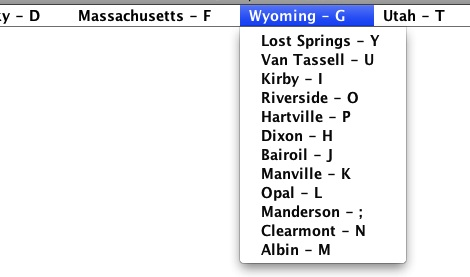
\includegraphics[width=\linewidth]{HKDDHartvilleZoom.jpg}
  \caption{Part of a dropdown menu, navigable by pressing and holding keys rather than with the mouse, used in the study; note the letters on each item.  Also note that the text is the same font and size as in the keyboard-card menus.}
  \label{fig:rcddmzoom}
\end{figure}

\subsubsection{Study Results}

The average selection times for the two different menu systems can be seen in \autoref{fig:averagetimes}.  Note that while outlier trials were removed (a trial was considered an outlier if its time was greater than 3*(Q3-Q1)+Q3, where Q1 and Q3 were the first and third quartile values; 0.55\% of trials were considered outliers), average times for participants who did not complete all 1440 trials were left in.  Averaged trial completion times for each block  are only complete for all participants and menu types in blocks 1-8.  One participant was only able to complete trials in blocks 1-8 for both menu types.  Two other  participants were only able to complete trials in blocks 1-10 using the dropdown menus, but were able to complete trials in all blocks using the keyboard-card menus.  The remaining 17 participants were able to complete trials in all blocks.

To analyze this data we first fit quadratic equations to the completion time data for each participant (with trial number as the independent variable and completion time as the dependent variable), leaving out times for trials where any participant was missing data, the result of which was complete data for 323 trials over blocks 1-8.  Paired t-tests on the coefficients of the fitted quadratics showed statistically significant (p = 0.0458) differences between the average second-order coefficients for keyboard-card and dropdown menus (i.e. there were statistically significant differences in the ``curviness'' of the data for the keyboard-card and dropdown menus).  In addition, we performed a repeated measures ANOVA on the average completion times for blocks 1-7 (where all participants completed all trials), which showed statistically significant differences between the two menu types (p = .044) as well as between the blocks (p < .001).

\begin{figure} [H]
  \center
  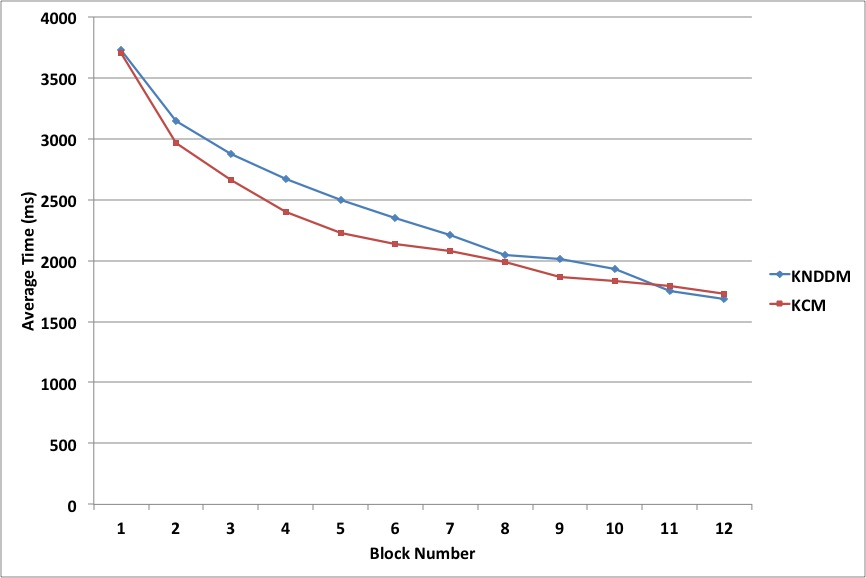
\includegraphics[width=\linewidth]{AverageTimes.jpg}
  \caption{Average trial completion times, in milliseconds, for the keyboard-navigated dropdown menus and keyboard-card menus in the study.  Note that data is only complete for blocks 1-8}
  \label{fig:averagetimes}
\end{figure}

Average error rates for each trial and menu type are shown \autoref{fig:errorrates}.  Overall error rates across blocks 1-7 for the dropdown menus and keyboard-card menus were 10.4\% and 8.4\% respectively, where errors were defined as the incorrect selection of a leaf in the menu hierarchy and the error rate for a block was calculated as $e/(e+t)$ where $e=$ the number of errors in the block's non-outlier trials and $t=$ the number of non-outlier trials in the block.  This difference was not statistically significant.  However, t-tests on the data for the 5th, 9th and 10th block differences did show statistical significance (p-values were .032, .008, and .049 respectively; note that 9th and 10th blocks exclude data for one participant).  Though a repeated measures ANOVA on the error rates for blocks 1-7 also failed to show statistical significance, fitting quadratics to the error rates for each participant at each block where data was available, and then performing t-tests on the coefficients \textit{nearly} showed statistical significance at the 5\% level for the quadratic and linear coefficients (p-values were .0544 and .0624 respectively)

Several interesting correlations can also be seen in the overall (i.e. across blocks) data for each participant.  Error rates for dropdown menus were correlated ($R=$0.718) with the error rates for keyboard-card menus and overall average times for dropdown menus were correlated ($R=$0.911) with overall average times for keyboard-card menus.  However, error rates and average times were negatively correlated for both dropdown menus and keyboard-card menus ($R=$ -0.510 and -0.479, respectively), so it appears that some participants chose to concentrate more on being accurate, at the expense of speed, and some chose to do the opposite.

In addition, the difference between the error rates for dropdown and keyboard-card menus was positively correlated with the error rate for dropdown menus (see \autoref{fig:errorratedifferences}) and the difference between the average times for keyboard-card and dropdown menus was positively correlated with the average times for dropdown menus (see \autoref{fig:timedifferences}).  In other words, participants whose error rates were higher made even more mistakes when using the dropdown menus, and participants whose average times were slow were even slower  when using dropdown menus.

\begin{figure} [H]
  \center
  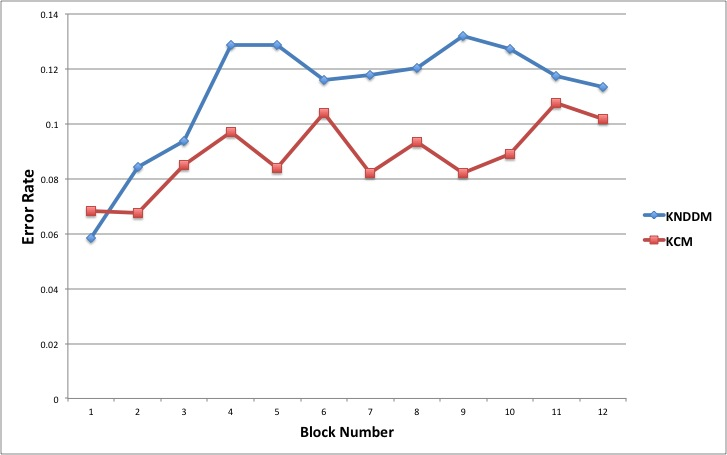
\includegraphics[width=\linewidth]{ErrorDataFixed.jpg}
  \caption{Error rates for the keyboard-navigated dropdown menus and keyboard-card menus in the study.  Note that data is only complete for blocks 1-8.}
  \label{fig:errorrates}
\end{figure}

\begin{figure} [H]
  \center
  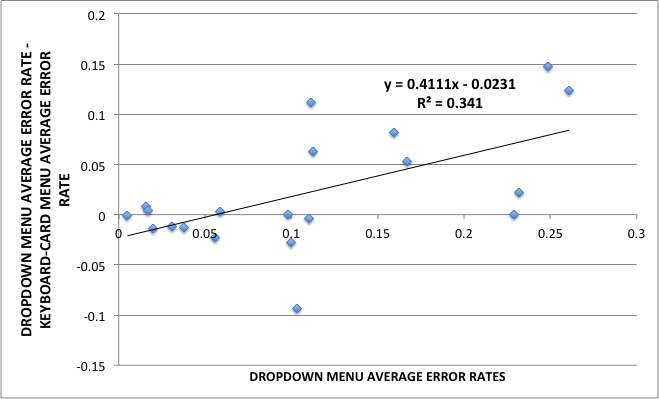
\includegraphics[width=\linewidth]{ErrorRateDifferences.jpg}
  \caption{The differences between the overall average error rates for dropdown menus and keyboard-card menus, for each participant, plotted against the error rate for dropdown menus.}
  \label{fig:errorratedifferences}
\end{figure}

\begin{figure} [H]
  \center
  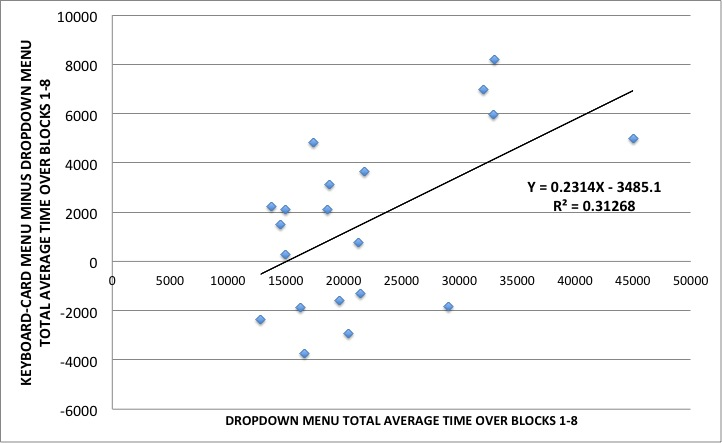
\includegraphics[width=\linewidth]{OverallAverageTimeDifferences.jpg}
  \caption{The differences between the overall average times for dropdown menus and keyboard-card menus, for each participant, plotted against the time for dropdown menus.}
  \label{fig:timedifferences}
\end{figure}

Results from the questionnaire can be seen in the table, where
\begin{itemize}
\item Q1=``How quickly do you feel you were able to become familiar with the menu item locations over the course of performing the trials?''
\item Q2=``At the beginning of the set of trials for this menu system, how quickly do you feel you were able to select menu items?'', and
\item Q3=``At the end of the set of trials for this menu system, how quickly do you feel you were able to select menu items?''
\end{itemize}
Ratings were given on a scale from 0=``Very Slowly'' to 9=``Very Quickly''.  Though the results were favorable for keyboard-card menus, t-tests did not reveal statistically significant differences between the average ratings (p-values given in the table). These results were not correlated with typing speed.

\begin{table}[h]
  \centering
  \begin{tabularx}{\linewidth}{ |X|X|X|X|X|X| }
  \hline
   & \bf{KCM Ave.} & \bf{KCM Std. Dev.} & \bf{DDM Ave.} & \bf{DDM Std. Dev.} & \bf{P-values} \\
  \hline
  \bf{Q1}  & 6.0  & 1.5  & 4.8 & 2.4 & .165  \\
  \hline
  \bf{Q2}  & 3.0  & 1.8  & 2.2 & 1.6 & .119  \\
  \hline
  \bf{Q3}  & 7.3  & 1.3  & 6.7 & 2.1 & .525  \\
  \hline
  \end{tabularx}  \caption{Questionnaire Results.}
  \label{tab:myfirsttable}
\end{table}

\subsubsection{Discussion}

The data supports the hypothesis that the keyboard-card menu's presentation makes rolled-chord shortcuts easier to learn than does the dropdown menu's presentation.  We further hypothesize, first, that the eventual convergence of the two curves in \autoref{fig:averagetimes} means that by the 12th block users memorized the 14 shortcuts (and so were not using either presentation), and second, that the initial divergence of the two curves indicates that the keyboard-card menu's presentation mostly helps users in finding and recalling shortcuts they have seen but not fully memorized.

Although in \autoref{fig:averagetimes} the separation between the curves appears to be small, it may be exaggerated considerably in more realistic applications by two factors.  First, the period in which users have seen menu items but have not yet memorized their locations (i.e. the middle section of \autoref{fig:averagetimes}) may be extended over a greater period of time (e.g. hours or days, rather than tens of minutes) affecting the number of menu selections needed for memorization.  Second, the effect of errors on the average selection times would likely be much greater, since only the time needed to make an error, recognize it, and make a correct selection is included in the \autoref{fig:averagetimes} data;  in realistic applications, the time to undo an error would also have to be included.

The negative correlation seen between error rates and average times shows users making a tradeoff between speed and accuracy.  However, the data seen in \autoref{fig:errorratedifferences} and \autoref{fig:timedifferences} suggests that use of a keyboard-card menu instead of a dropdown menu can help both users who prefer speed to accuracy and users who prefer accuracy to speed.

Many issues surrounding keyboard-card menus remain unexplored.  For instance, some participants disliked the use of bright colors.  Would refining the system improve performance?  Another color-related refinement would be to use different colored/textured cards for each submenu (in the study, all sub-cards in the second level were red).  Other important questions include: Does the menu actually encourage first time users of a system to use the shortcuts? What happens when icons instead of, or in addition to, labels are used? What is the best way to map a hierarchy to the menu? What happens when three finger shortcuts are used?  Can keyboard-card menus' presentation be effective with other sorts of shortcuts?

\subsubsection{Conclusion}

While selecting from a large set of menu items in an efficient manner is certainly possible, expecting users to learn how to do so using traditional shortcuts displayed in dropdown menus is often unrealistic.  In order to open up new realms of computer applications to a wider range of users (college students typing of mathematics at the computer, for instance), we are rethinking shortcuts and, in particular, how to present them.  We have developed keyboard-card menus, and have tested them against dropdown menus as a way of presenting how to enter shortcuts, using rolled-chords as our shortcut choice in the experiment.  Our data shows that keyboard-card menus, taking advantage of increasing amounts of available screen space with their keyboard-shaped presentation, can be more effective than a presentation based on dropdown menus as a method for presenting large numbers of shortcuts in an easy-to-learn way. 

\subsubsection{Acknowledgements}

We would like to thank our participants for their time and effort.  This research was supported by NSF award CCF-1250306.



%%============
\subsection{``Propositional Logic Syntax Shortcuts''}
%%============

Like Proof Transitions, the ``{\bf Proposition Logic Syntax Shortcuts}'' CoqEdit extension combines two ideas.  The first idea is keyboard-card menus, described above. One reason I would like to develop Propositional Logic Syntax Shortcuts is to see if keyboard-card menus can be successfully integrated into a real application.

The second idea incorporated into Propositional Logic Syntax Shortcuts is ``{\bf Syntax Tree Highlighting}''.  Syntax Tree Highlighting  is text highlighting of parse-able text document (e.g. program) where
\begin{itemize}
\item only text of a node in the concrete syntax tree of the document
\item the children of the node are shown as distinct sections of highlighting
\item something, e.g. a line under the highlighting, shows which child nodes are leaf nodes
\item the highlighting of one of the non-leaf children, if there are any, indicates that it is ``selected''
\item the user can navigate the syntax tree  by moving the indication of selection from non-leaf node to non-leaf node and by moving the highlighting to the selected non-leaf child node or the parent of the node with highlighting.
\end{itemize}
Syntax Tree Highlighting can be useful in understanding the syntax of text (which, of course, is generally a prerequisite for understanding its semantics), and may be particularly helpful in resolving ambiguities that result when the author of the text did not include parentheses.  Ambiguities of this sort can occur in in many languages, which suggests that Syntax Tree Highlighting may be widely useful.  A good example is a math problem that, according to an article in \textit{Slate} magazine\cite{HaelleMarch122013}, has been circulating on \textit{Facebook}.  The problem is to compute
\begin{equation}
6 \div 2(1 + 2)
\end{equation}
The fact that there even is a \textit{Slate} story on this problem indicates that it really is ambiguous, despite attempts, described in the story, at establishing a standard algorithm.  Computer scientists and programmers encounter such ambiguities frequently when reading and writing programs, especially in languages new to them.  The situation with Coq is especially bad, in part because Coq allows users to define their own ``notations'' and to give them precedence levels and directions of associativity (e.g. ``\texttt{+}'' and ``\texttt{/\symbol{92}}'' are notations).

Even when there is no real ambiguity that needs to be resolved, Syntax Tree Highlighting could make code more readable.  For instance, given fully parenthesized text, finding matching pairs of parentheses can be difficult, and finding all of the ``next level'' parentheses within a given pair is even harder.  ``Pretty printing'' techniques, involving indentation, can also help make code more readable, but keeping indentation levels straight can still be difficult, if the text file in question is long, and there is only so far over one can indent without having to scroll over.  Furthermore, in many cases coders must deal with code written by other coders or generated by a computer (e.g. the terms generated in Coq by sequences of tactics), and in these cases there are generally no guarantees about parenthesization or pretty printing. 

Syntax Tree Highlighting may also be useful in selecting important sections of text (compare moving its highlighting with selection in the usual character-by-character or line-by-line way) to manipulate (e.g. rewrite, cut, copy, paste over) and ``inspect'' these sections.  In the case of Coq, ``inspecting'' these sections could mean type checking or evaluating them.

\autoref{fig:sth} gives an example of what Syntax Tree Highlighting might look like in Coq.  In (a) through (d), we see the highlighting moving through the nodes of the syntax tree of the term, going first to the right-most child node and then to the left-most.  Along the way, a few things are made clear:
\begin{itemize}
\item the scope of ``\texttt{forall x : G,}'' extends all the way to the end of the term.
\item ``\texttt{=}'' binds more tightly than ``\texttt{/\symbol{92}}''
\item ``\texttt{X}'' is actually an infix operator (probably declared earlier in the file), not an argument to ``\texttt{x}''
\end{itemize}
In (e), we see (d)'s selected child node replaced with a new term, ``\texttt{a}'', demonstrating Syntax Tree Highlighting could be used in manipulating text.  As noted earlier, this highlighting could also be used to inspect nodes so, for instance, in (a) the user might see ``\texttt{Prop}'' displayed in some other window to indicate that ``\texttt{forall x : G, x X inv x = e /\symbol{92} inv x X x =  e}'' has type \texttt{Prop}.

\begin{figure} [H]
  \center
  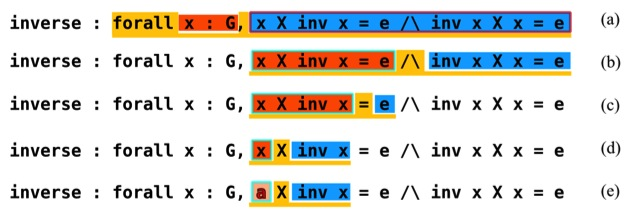
\includegraphics[width=\linewidth]{syntaxtreehighlighting.jpg}
  \caption{Example of Syntax Tree Highlighting in Coq.}
  \label{fig:sth}
\end{figure}

Propositional Logic Syntax Shortcuts involves, on the one hand, some scaling back of my full ambitions for Syntax Tree Highlighting in Coq, and, on the other hand, an implementation of a generalizable form of coding and perhaps a more effective use of keyboard-card menus than I had originally envisioned.   For this plugin, I will be considering only a subset of Coq's language that may be used in doing ``Fitch-style'' proofs in classical propositional logic, as presented in the popular textbook \textit{Logic in Computer Science: Modelling and Reasoning about Systems} by Michael Huth and Mark Ryan \cite{huth2004logic}.  Proofs in this style do not involve turnstiles or colons.  Instead, they are lists of formulas where each formula is either a premise or a hypothesis, or follows, according to an inference rule from a given set of such rules, from zero or more formulas at earlier positions in the list.  In \cite{huth2004logic} the formulas in these lists are generally written no more than one to a line, each with a short justification (e.g. the name of an inference rule and the line numbers formulas used), and with (possibly nested) boxes surrounding formulas to show where it is to be assumed that a hypothesis, at the top of the box, is valid (i.e. to show the scope of the hypothesis).   Although Coq is not really designed for writing proofs in this style, in \autoref{fig:plss1} I show how to imitate it within a Coq .v file.  Note that ``Fact'' is a synonym for ``Lemma'' or ``Theorem'', that the proof/hypothesis names l1, l2, l3, stand for line numbers, that the simple proofs are applications of axioms or theorems that correspond to natural deduction inference rules given in \cite{huth2004logic}, and that Coq's section mechanism, along with indentation, takes the place of boxes.  While restricting Coq in this way restricts Coq's power enormously, it may also make Coq more accessible and useful to the many students studying propositional logic using books like \cite{huth2004logic}. 

The main idea I hope to demonstrate with Propositional Logic Syntax Shortcuts is that, by using a combination of Syntax Tree Highlighting and keyboard-card menus, code can be efficiently written by building it up using the rules of a grammar.  If one just considers a propositional logic formula, the sequence of states that the formula goes through might look like 
\begin{enumerate}
\item \texttt{[?]}
\item \texttt{[?] -> ?}
\item \texttt{([?] -> ?) -> ?}
\item \texttt{(A -> [?]) -> ?}
\item \texttt{(A -> ([?] -> ?)) -> ?}
\item \texttt{(A -> (B -> [?])) -> ?}
\item \texttt{(A -> (B -> C)) -> [?]}
\item \texttt{(A -> (B -> C)) -> [?] -> ?}
\item \texttt{(A -> (B -> C)) -> ([?] -> ?) -> ?}
\item \texttt{(A -> (B -> C)) -> (A -> [?]) -> ?}
\item \texttt{(A -> (B -> C)) -> (A -> B) -> [?]}
\item \texttt{(A -> (B -> C)) -> (A -> B) -> A -> [?]}
\item \texttt{[(A -> (B -> C)) -> (A -> B) -> A -> C]}
\end{enumerate}
where  ``\texttt{?}'' is a placeholder for text that needs to be added, and the square brackets represent the location of the Syntax Tree Highlighting.\footnote{This process of filling in placeholders is actually what is going on behind the scenes when tactics are used--the displayed goals are the types for placeholders within the term being constructing.}  While the details of exactly which commands to arrange where within a keyboard-card menu for the Propositional Logic Syntax Shortcuts extension remain to be determined, moving through the above states could involve just selecting from four menu items perhaps labeled ``\texttt{A}'', ``\texttt{B}'', ``\texttt{C}'', and ``\texttt{[?] -> ?}'' (deciding on reasonable menu item labels is part of the project).  As a possibly more natural alternative, users could move through a sequence of states
\begin{enumerate}
\item \texttt{[?]}
\item \texttt{[A]}
\item \texttt{A -> [?]}
\item \texttt{A -> [B]}
\item \texttt{A -> (B -> [?])}
\item \texttt{A -> (B -> [C])}
\item etc.
\end{enumerate}
using additional menu items that might be labeled ``\texttt{[A]}'', ``\texttt{[B]}'', ``\texttt{[C]}'', and ``\texttt{\_ -> [?]}''.  In \autoref{fig:plss1}, \autoref{fig:plss2}, and \autoref{fig:plss3} we see how a user could also use navigate through the file's overall syntax tree to delete a particular formula. The navigation and deletion commands could also be entered using items in the keyboard-card menu.  N.B.: the available menu items (i.e. ones that are not ``grayed out'') can be restricted so that, for instance, users cannot replace the entire expression \\``\texttt{Fact l3 : phi \bstt/ \tildett{}phi. Proof. apply (or\_intro\_l l2). Qed. }''  with \\``\texttt{[?] -> ?}''.

Two final comments.  First, writing code by selecting and combining grammatical components is not particularly new.  A couple of examples are \textit{Scratch}\cite{Scratch}, an environment for developing programs by dragging and dropping interlocking pieces, and the interfaces of various graphical typesetting tools (e.g. that of \textit{Mathematica}\cite{Mathematica}).   What \textit{is} new is its combination with keyboard-card menus to provide a fast, from-the-keyboard, way of creating programs that I hope can smooth the transition from novice to expert programmer.

Second, writing code in this way may be viewed as a continuation of a general effort to stop programming errors early--an effort spearheaded by Coq's advanced type system.    Types and type checking are used to move the detection of errors from run time to compile time.  Integrated development environments nowadays often auto-compile code so that programmers can spot errors almost immediately after they type a character into a buffer.  Coding at the level of grammatical components can stop some errors before they even reach the buffer.  

\begin{figure} [H]
  \center
  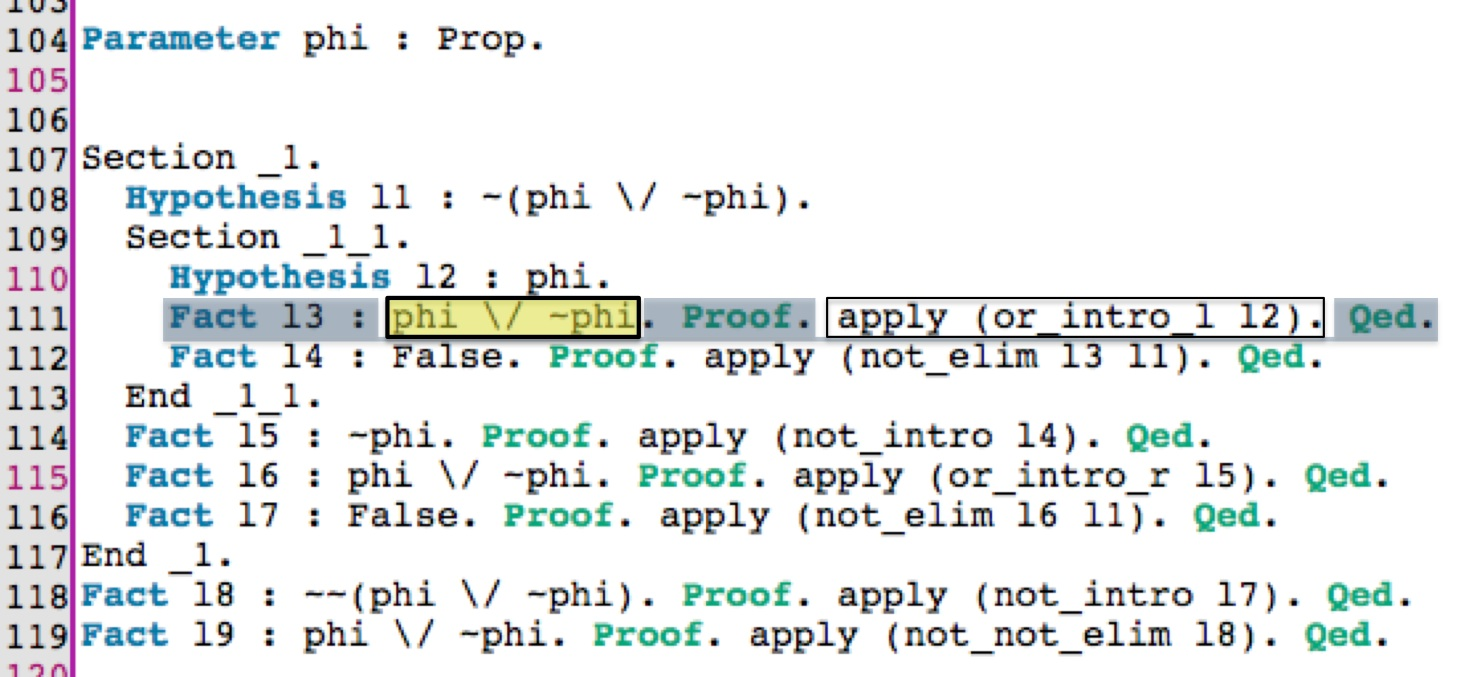
\includegraphics[width=\linewidth]{PLSS_1.jpg}
  \caption{Syntax Tree Highlighting for Propositional Logic Syntax Shortcuts.  Note how the text corresponds to a Fitch-style proof with the two sections corresponding to boxes, one nested in the other.}
  \label{fig:plss1}
\end{figure}

\begin{figure} [H]
  \center
  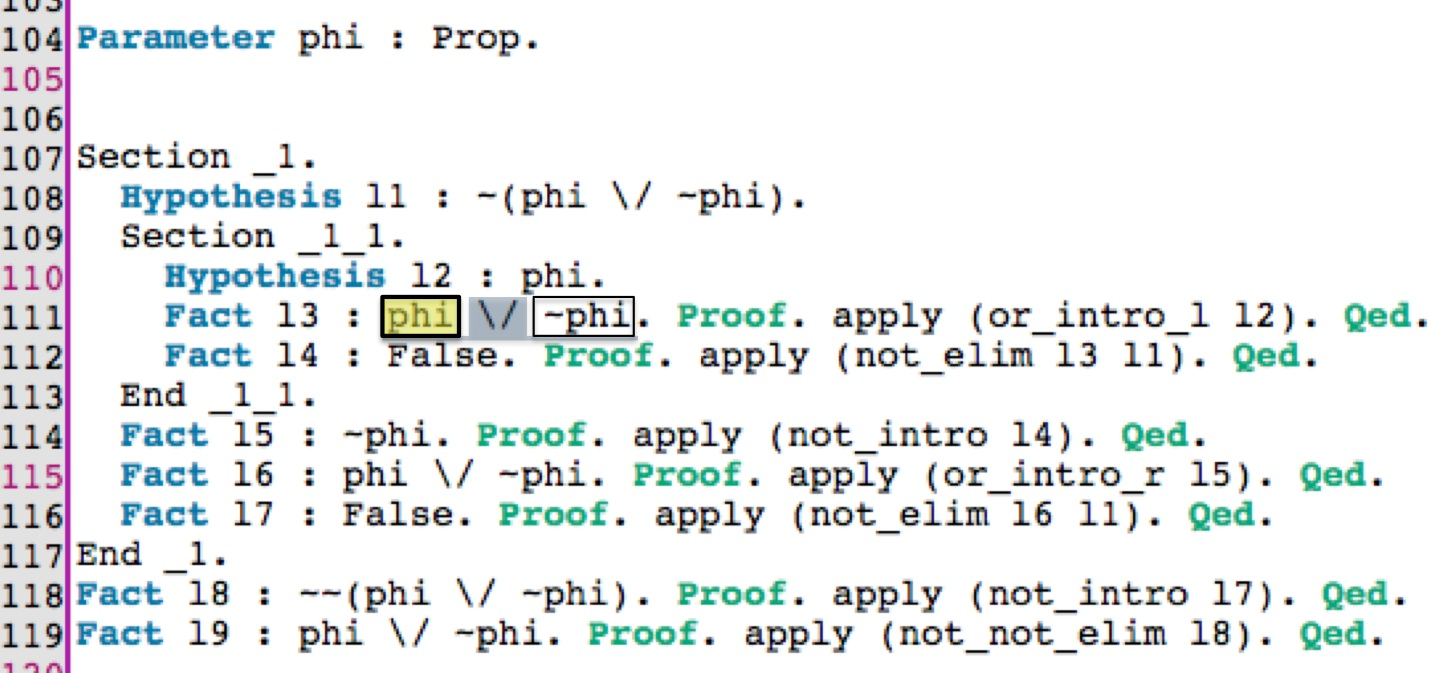
\includegraphics[width=\linewidth]{PLSS_2.jpg}
  \caption{Syntax Tree Highlighting for Propositional Logic Syntax Shortcuts, with highlighting moved from \autoref{fig:plss1}.}
  \label{fig:plss2}
\end{figure}

\begin{figure} [H]
  \center
  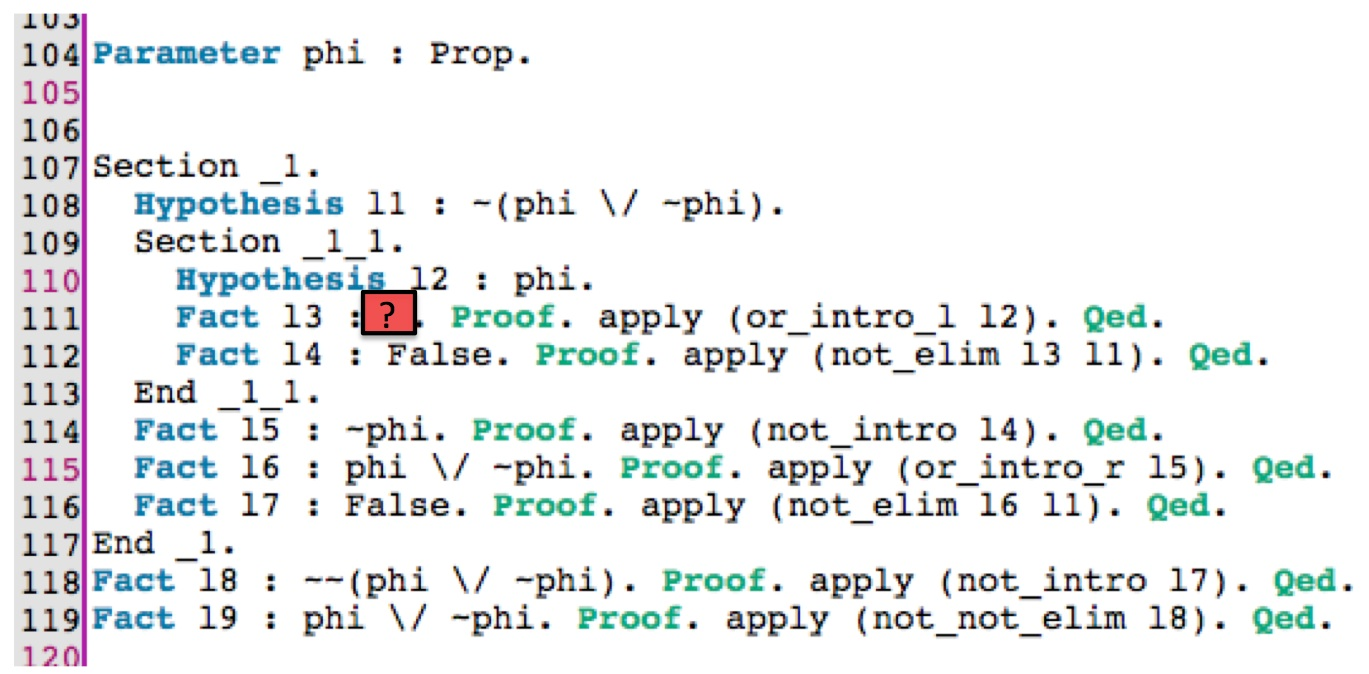
\includegraphics[width=\linewidth]{PLSS_3.jpg}
  \caption{Syntax Tree Highlighting for Propositional Logic Syntax Shortcuts, with highlighting moved from \autoref{fig:plss1}}
  \label{fig:plss3}
\end{figure}



%%================================
\subsection{Extension Testing}
%%================================

Testing the Proof Previews and Proof Transitions extensions with participants (university students) will be combined in a single experiment, already approved by the University of Iowa IRB.  The rough plan for the experiment is to first take participants through a tutorial on proving theorems in propositional and first-order logic with Coq.  Participants will then walk through a pair complicated proofs, using Proof Transitions for one and un-extended CoqEdit for the other, and will be asked to give detailed explanations of what they see.  These explanations will be recorded and graded later.  Finally, participants will be given two sets of lemmas to attempt to prove, one with Proof Previews and the other without, and the amount of time they need (or the number they are able to prove) will be recorded.  For both the Proof Transitions and the Proof Previews, ordering of problems and pairing of problem to extension will be balanced across participants, and informal feedback will be acquired along the way.\footnote{Some informal feedback from Coq users and potential users, indicating that our ideas seem reasonable, has already been acquired.}

For the now at least, I am considering testing of Propositional Logic Syntax Shortcuts with human subject to be beyond the scope of the proposed dissertation.  However, given that it will be developed with Huth and Ryan's textbook in mind (which has been used at the University of Iowa, among other places), the plugin should certainly lend itself to testing in a classroom setting.

%%=======================================================================================
\section{Timeline for Research}
%%=======================================================================================

A tentative schedule:
\begin{itemize}
\item Completion of the revised version of CoqEdit, the Proof Previews plugin, and the Proof Transitions by the end of August 2013.
\item Experiment with Proof Previews and Proof Transitions in September and October 2013 (I will be acting in a supervisory role here, and in getting the experiment set up).
\item Development of Propositional Logic Syntax Shortcuts in October 2013 through January 2014
\item Further refinement of plugins, dissertation writing, February through April 2014
\item Dissertation defense, May 2014
\end{itemize}

%%=======================================================================================
\chapter{Related Work}
%%=======================================================================================

The need for effective theorem prover user interfaces has been recognized for over 20 years (e.g. \cite{Thery:1992:RTP:142868.143760}) and a series of conferences has even been organized to address this need specifically.\footnote{See http://www.informatik.uni-bremen.de/uitp/ for more information} Many interesting and helpful ideas have been proposed, both for Coq and for related systems.  These ideas vary widely and include integration of Coq, and other theorem provers, with dynamic geometry software \cite{narboux2007graphical,quaresma2007geothms}, easier-to-read declarative languages for proof scripts \cite{corbineau2008declarative}, using wikis for creating proof repositories \cite{corbineau2007cooperative}, and automating the process of using libraries \cite{asperti2010some}.

One approach taken to improve theorem prover user interfaces has been ``Proof by Pointing''\cite{bertot1994proof}, an algorithm to build a proof tree by pointing to portions of a goal.  This was implemented in the \textit{CtCoq} interface \cite{bertot1996ctcoq}, again, later, in the Java-based Pcoq interface \cite{amerkad2001mathematics} and also in the \textit{Jape} system \cite{bornat1999animating}.  Note that some schemes for writing and displaying proofs, notably Fitch style proofs, to not display hypotheses with their conclusion, which may lead to ambiguity when using Proof by Pointing \cite{bornat1997displaying}. 

An example of a recent project is \textit{Panoptes} \cite{farmer2009panoptes}, which allows visualization of proofs produced by the IMPS Interactive Mathematical Proof System.  The system has numerous features allowing users to zoom in on parts of the graph, collapse nodes, rearrange the positions of nodes, label and highlight nodes, and inspect details associated with nodes using pop-up windows.  while these features allow the user to manipulate the presentation of a proof, they do not allow the user to manipulate the proof itself--to change the proof, one must use an Emacs-based environment.

Another significant project is an interactive visualizer for the \textit{ACL2} theorem prover\cite{ACL2}, described in \cite{bajaj2003interactive}.  This tool allows for visualization at three different levels.  It does so first at the level of relationships between theorems and their proofs (the directed acyclic graph describing which lemmas from which libraries are used to prove a given theorem).  Next, it shows a proof tree, similar to the visualization given in section \ref{prooftransitions}, where a node represents a statement that is being proved using the node's children.  Color coding is used here to indicate the action taken by the prover at a node, and the tree is represented using three-dimensional ``cone trees.''  The contents of the individual nodes, as text, can also be displayed alongside this tree.  At the third level, this text's syntax tree can be visualized (as lines connecting points again, though in a more usual two-dimensional arrangement, and still in contrast with the Syntax Tree Highlighting discussed above).  Selecting text at this level will highlight the corresponding portion of the tree visualization.  The system also supports textual pattern matching, where the degree of matching is indicated by the color of the text and the tree visualization.  Both at this level and at the proof structure level (i.e. the second level) the system is capable of zooming and panning, and, at the proof structure level, rotating is also possible.

A few other significant projects aiming to improve the presentation of machine-checked proofs include \textit{Proviola}, which allows users to move through a proof script displayed on a web page and view the results that Coq would produce \cite{tankink2012narrating}; an ``Interactive Derivation Viewer'' for visualizing derivations written in the TPTP language \cite{trac2007interactive}; the LOUI interface for the OMEGA proof assistant, featuring graphical visualization, term browsing, and natural language proof presentation \cite{siekmann1999loui}; and the Tecton system, featuring tree visualization combined with hypertext navigation of nodes \cite{kapur1994overview}.  Theoretical and methodological work has also been done and can be seen in \cite{eastaughffe1998support,bertot1998generic,luth1999functional,volker2004thoughts,geuvers2009proof}, and \cite{luth2009user}.  Work aimed at making ITPs more suitable for novices and educational settings includes \cite{tsovaltzi2003approach,meier2004adaptable,narboux2007graphical,billingsley2007student,dillinger2007acl2s,hendriks2010teaching,schreiner2009risc} and \cite{pierce2010proofassist}.

In addition to previous work specifically on theorem prover user interfaces, it is important to consider more general human-computer interaction research and research on software development tools.  Starting with the latter, one can consider the data of \cite{murphy2006java} showing that the Eclipse IDE's ``rename,'' ``move,'' ``extract'', and ``inline'' refactoring commands are in fact used by many programmers and are frequently invoked via key bindings.  The data also shows that a large percentage of \textit{all} commands executed by developers using the IDE extensively were invoked via key bindings, and one of the top commands was ``content assist'', which suggests possible text to insert (similar to Proof Previews, though it does not show the effects of evaluating this text).

In addition to IDEs, we may consider software visualization tools:  \cite{bassil2001software} report on a survey of users of software visualization tools such as \textit{daVinci} (now called \textit{uDraw(Graph)}), \textit{GraphViz}, \textit{Grasp} (now \textit{jGrasp}, and \textit{Tom Sawyer Software}--more than 40 different tools altogether.  Some of the ``functional aspects'' of the software visualization tools that were considered most useful, and that might also have useful analogs in theorem prover user interfaces, were ``search tools for graphical and/or textual elements'', ``hierarchical representations'' and ``navigation across hierarchies'', ``use of colors'', and ``easy access, from the symbol list, to the corresponding source code.''  Among functional aspects considered least useful were ``3D representations and layouts, and virtual reality techniques'' and ``animation effects'', though the later was considered ``quite useful'' when the software was implemented in a declarative language.  Software visualization tools were considered beneficial in increasing productivity and managing complexity, and were considered particularly important in the ``software comprehension process.''

A survey and taxonomy of software visualization is presented in \cite{caserta2011visualization}.  Similar to \cite{bajaj2003interactive}, it divides tools into three groups according to their use at three different levels of abstraction: line, class, and architecture.  They also differentiate between tools used for visualizing code at a particular time and those that allow for visualization of the evolution of software.  Many of the techniques used by these tools could be applied to visualization for interactive theorem provers.  \textit{Seesoft} \cite{eick1992seesoft}, for instance, miniaturizes lines of code with lines of color-coded pixels, and \textit{sv3D} \cite{marcus20033d} extends this idea using three-dimensional arrays of blocks where information about lines of code is encoded in the height and color of the blocks.  Other techniques potentially useful for interactive theorem prover user interfaces include using animation and color gradients to show the direction of relationships between software components \cite{alam2007evospaces,holten2006hierarchical} and using texture and 3D object primitives called ``geons'' to encode additional information \cite{holten2005visual,irani2001using}.

The more general human-computer interaction literature on tree visualization is quite extensive--many techniques have been developed.  Four different ``common layouts'' are listed in \cite{holten2006hierarchical}: rooted tree (the node layout presented, for instance, in \autoref{fig:similarnodes}, with child nodes arranged on a horizontal line above or below their parents), radial trees (nodes of each level of the tree are arranged in concentric circles, with the root node at the center, its children at the first circle out, their children at the next circle out, etc.), balloon trees (each parent's child nodes are arranged radially around the parent), and treemaps (which divide a rectangle into smaller and smaller rectangles with the largest rectangle representing the root of the tree and the smallest representing the leaves, and where division of the rectangles switches between using horizontal and vertical lines when going between tree levels; these were developed in \cite{shneiderman1992tree}).  These common layouts have been extended in various ways.  For instance, \cite{nguyen2002space} describes a space-optimized version of balloon trees and \cite{van1999cushion} describes the the addition of gradients to the rectangles in treemap visualizations, making the structure of the tree easier to see.

\cite{katifori2007ontology} presents an extensive review of tree visualization techniques.  Along with classifying visualizations as 2D or 3D (or 2.5D when no movement in or manipulation of a 3D visualization is allowed), it divides the visualizations into six overlapping categories: indented list, node-link and tree, zoomable, space-filling, focus+context or distortion, and three-dimensional information landscapes.  Indented lists can be seen in file system browsers, e.g. \textit{Microsoft Windows}' \textit{Explorer}, the rooted and radial trees mentioned in \cite{holten2006hierarchical} as common layouts are ``node-line and tree'' type, and treemaps are an example of the space-filling type.  An example of a zoomable visualization is \textit{Grokker} \cite{rivadeneira2003study} which allows users to click and expand nested circles.  An example of the focus+context or distortion category is the \textit{Hyperbolic Browser} \cite{lamping1996hyperbolic} which magnifies and centers on the area around a selected node in a radial layout.  An example of a three-dimensional information landscape is the \textit{Harmony Information Landscape} \cite{eyl1995harmony}.



%=======================================================================================
\chapter{Conclusion and Acknowledgements}
%=======================================================================================

I hope to have made several points in this proposal.  First, that this is important work, both because the Coq interactive theorem prover is an important tool that could benefit significantly from improved user interfaces and because many of the ideas generalize to other forms of coding.  Second, that as an intellectual challenge this work is non-trivial, not only because of the normal programming problems that must be overcome but because designing good user interfaces for complicated systems, which includes the identification of tractable problems and the testing of potential solutions, is non-trivial.  Finally, that, despite this non-trivial nature, the work can be accomplished.

Much of the work presented has been supported by NSF award CCF-1250306.  I also give special thanks to my advisor, Professor Juan Pablo Hourcade, Professor Aaron Stump, and Harley Eades, for working on this project with me, and to my committee.

%===================================================================================================
\bibliographystyle{plain}
\bibliography{refs}

\end{document}  